\onlyinsubfile{\setcounter{section}{2}}
\section{Descriptive statistics}\notinsubfile{\label{sec:data}}

\par For the statistical analysis in this paper, I use the RAND Longitudinal version of the Household Retirement Survey (HRS) public data. I focus on the years 2002-2022; as this time horizon was filled with many economically relevant events (GFC, Covid), we can be creative regarding how to assess the accuracy of the data measured here. This is useful because, although there are many sources of income data to compare resuults to, there are less counterparts like this for return measures. The variables of interest fall into the categories: i) income, ii) wealth and portfolio composition, iii) returns, iv) trust, v) demographics, and vi) other controls.


\subsection{Income}

\par First, I use two measures of income: labor and total. Labor income is a narrow measure only capturing earnings and unemployment income. Total income is a more broad measure including retirement and capital income. Table ~\ref{{fig:income_over_time}} shows that, for the time period, mean incomes are relatively flat over the period. Moreover, the discrepancy between mean labor and total income is likely driven by the oversampling if older and retired households by the HRS.  

\begin{figure}[H]
\centering
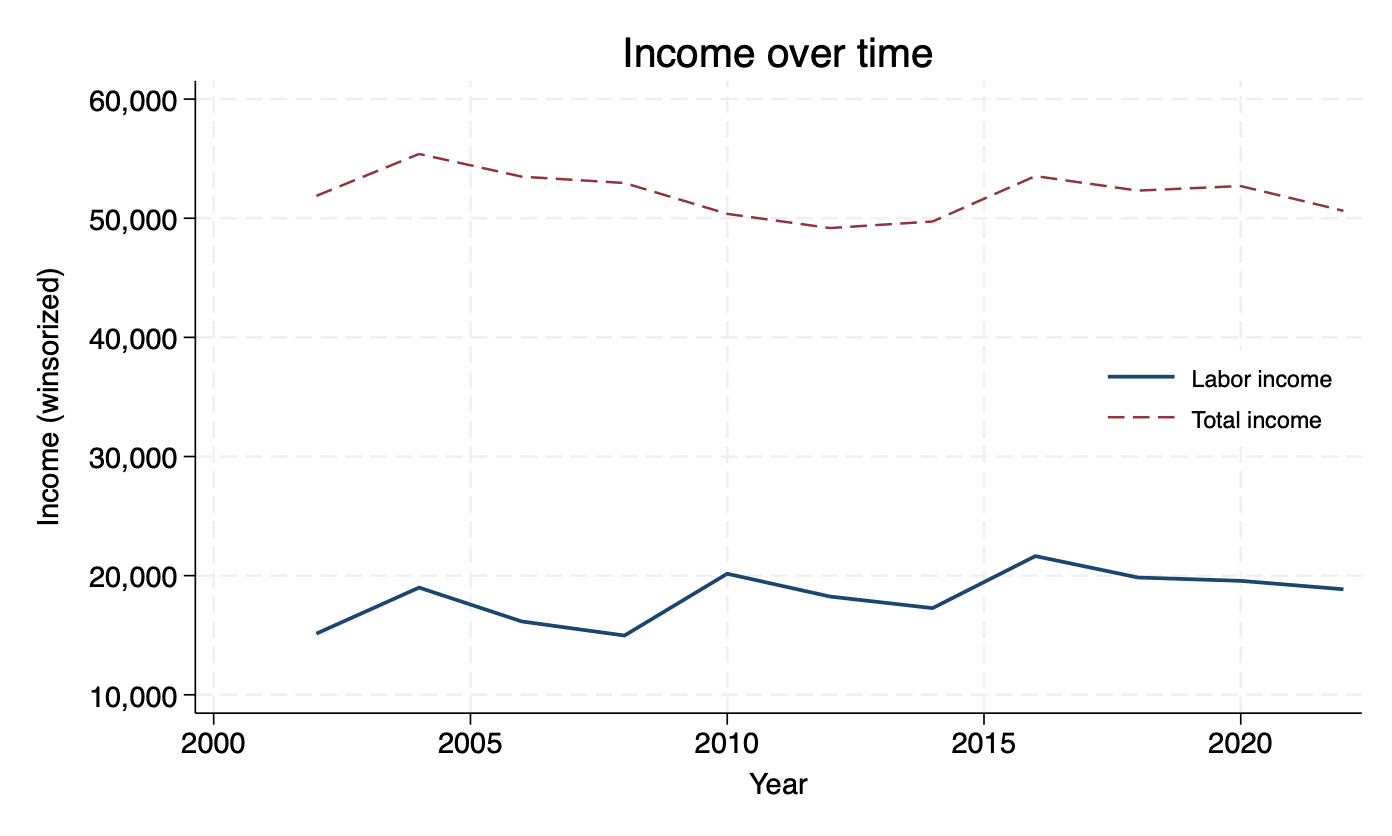
\includegraphics[width=0.8\textwidth]{../../Code/Descriptive/Figures/income_over_time.png}
%\caption{Income over time}
\label{fig:income_over_time}
\end{figure}
\FloatBarrier

\par In particular, I pooled the observations of the survey together to get a sense of the distribution of incomes measured in the survey. This is captured by Table~\ref{tab:income_final_tabstat}.

\inputtable{../../Code/Descriptive/Tables/income_final_tabstat.tex}
\label{tab:income_final_tabstat}

\par An important finding in the literature on earnings in the U.S. is that it is generally hump-shaped over the lifecycle. It is a good sign then that figure ~\ref{fig:income_by_agegroup_2020}

\begin{figure}[H]
\centering
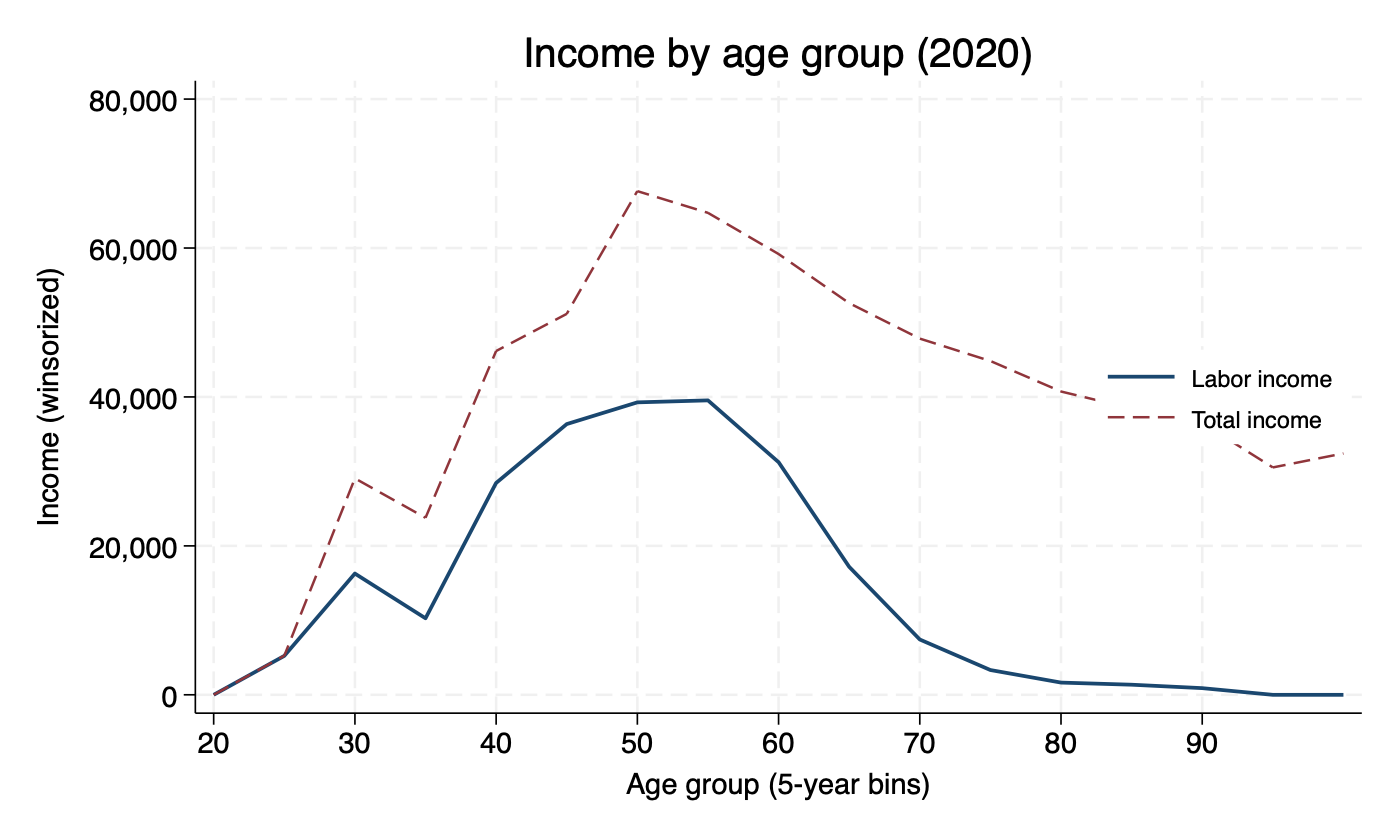
\includegraphics[width=0.8\textwidth]{../../Code/Descriptive/Figures/income_by_agegroup_2020.png}
%\caption{Income by age group (2020)}
\label{fig:income_by_agegroup_2020}
\end{figure}
\FloatBarrier

\par Another empirical finding in the literature on earnings is that on average individuals with more education earn higher income. The trend captured in Table~\ref{tab:income_mean_by_educgroup_real_win} suggests that the earnings data is in line with one would respect regarding earnings for a representative survey in the U.S.\footnote{ Although the HRS oversamples older households, I use the provided the respondent-level weights for this interpretation of the summary statistics of the data.}

\inputtable{../../Code/Descriptive/Tables/income_mean_by_educgroup_real_win.tex}
\label{tab:income_mean_by_educgroup_real_win}

\begin{figure}[H]
\centering
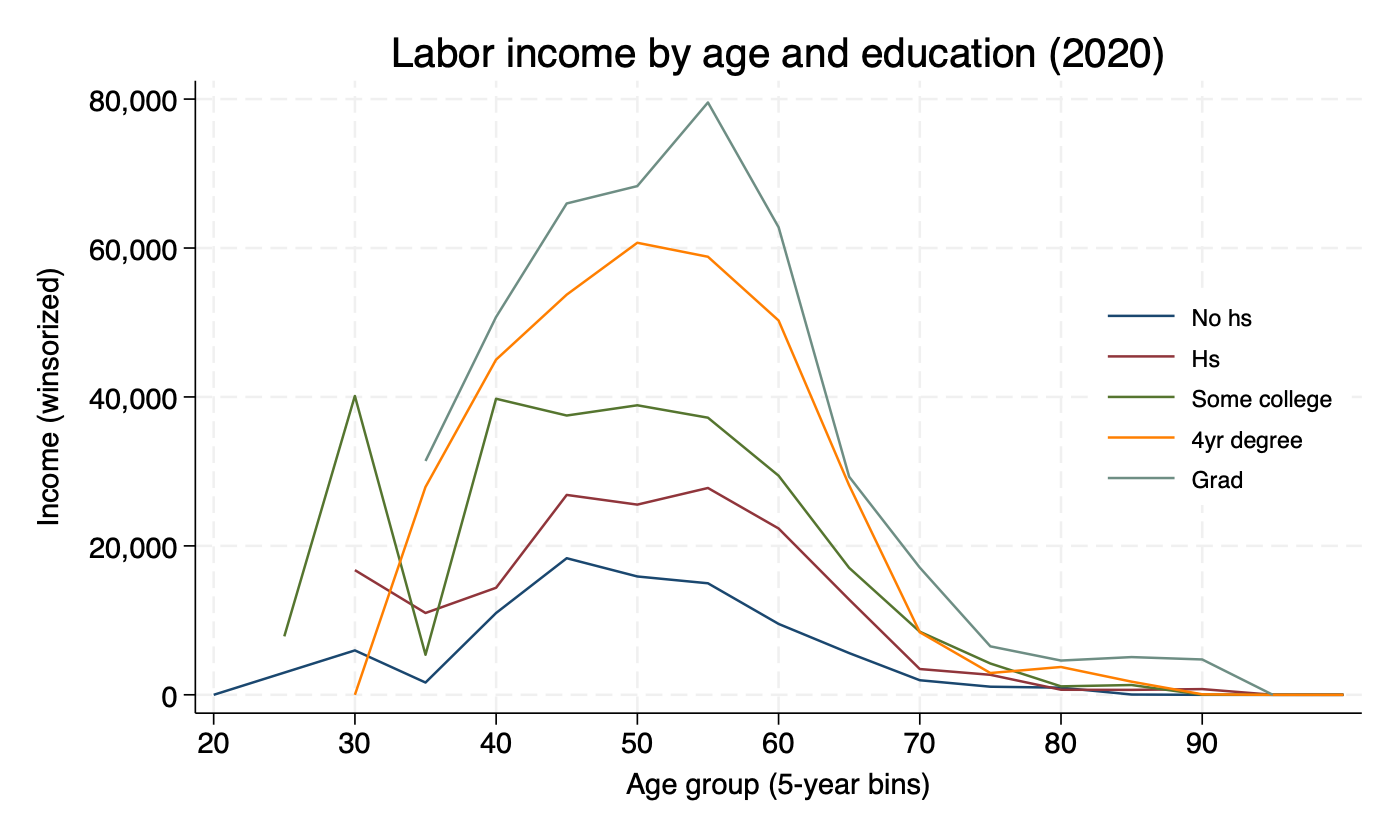
\includegraphics[width=0.8\textwidth]{../../Code/Descriptive/Figures/labinc_by_age_educ_2020.png}
\caption{Labor income by age and education (2020)}
\end{figure}
\FloatBarrier

\begin{figure}[H]
\centering
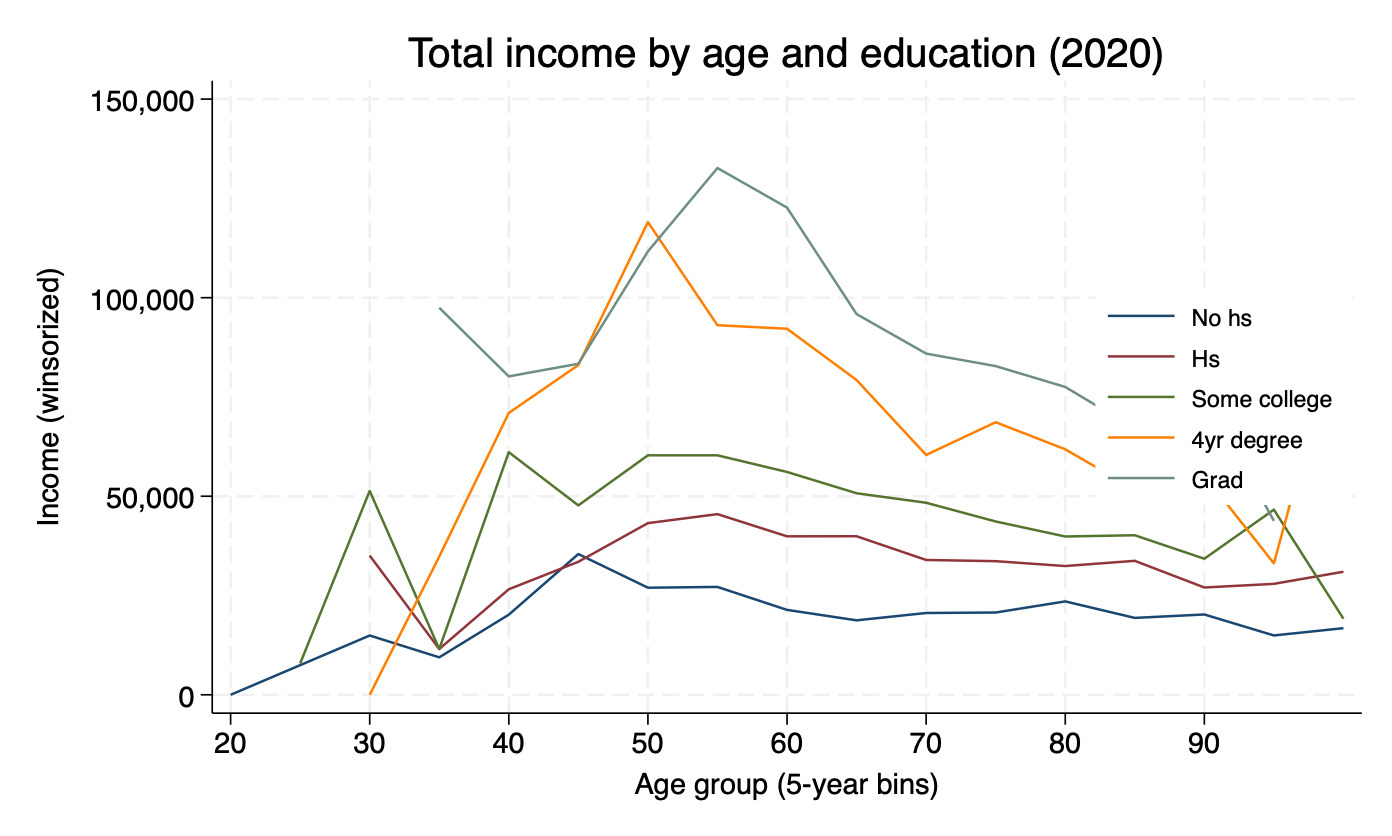
\includegraphics[width=0.8\textwidth]{../../Code/Descriptive/Figures/totinc_by_age_educ_2020.png}
\caption{Total income by age and education (2020)}
\end{figure}
\FloatBarrier

\subsection{Asset classes and portfolio definitions}

\par The HRS asks a number of questions aimed at measuring household wealth and portfolio composition in the sample. I collect data on i) \textbf{interest income and dividends}, ii) \textbf{capital gains}, iii) \textbf{net investment flows}, and iv) \textbf{previous period wealth holdings}, all of which are necessary to define the desired measure of household returns. Since population-level administration data on these objects for individual taxpayers is not available in the U.S., it is important to understand each component needed in the return calculation. This will help to determine whether or not our measured distribution of returns in this dataset is sensible. To understand what portfolios are accruing returns, we will let the structure of the HRS questions guide how we define returns to specific asset classes (and collections of them) that the survey collects data for.

\subsubsection{Interest income and dividends}

\par The HRS RAND longitudinal file has a distinctive way in which interest income and dividends received on major asset classes, like stocks and bonds, private business, and real estate, is measured. In particular, there is a variable in the survey which measures \say{household capital income}:

\begin{itemize}
  \item $\ldots$is the sum of household capital income received over the last calendar year, including business or farm income, self-employment earnings, gross rent, dividend and interest income, trust funds or royalties, and other asset income.
  \end{itemize}

  This particular feature of the data is the driving factor for the key modeling assumptions of this paper regarding measuring returns: asset classes are defined as narrowly as they can be given observation of interest income and dividends on those assets. For example, although we see capital gains for stocks, business, bonds, and real estate, we do not observe interest income or dividends on these assets individually. Thus, the narrowest asset class defined in this paper will be called \say{core assets} and will be comprised of these assets.

  \par The RAND version of the data offers a number of variables measuring pension and annuity income as well as other forms of retirement income. I use this to construct a measure of returns to retirement assets and to define a broader notion of portfolio returns by considering returns to core and retirement assets.

  \par A key assumption is that there are no interest income or dividends earned on residential assets\footnote{Or on any of the asset classes for which capital gains are available for.}. With this assumption, we can consider interest income and dividends on the entire portfolio as the same as interest income and dividends on the portfolio with just core and retirement assets. Thus, to compute a measure of returns to net wealth, I need to add in the remaining available capital gains per asset class (for those that receive no interest income). 

\begin{figure}[H]
\centering
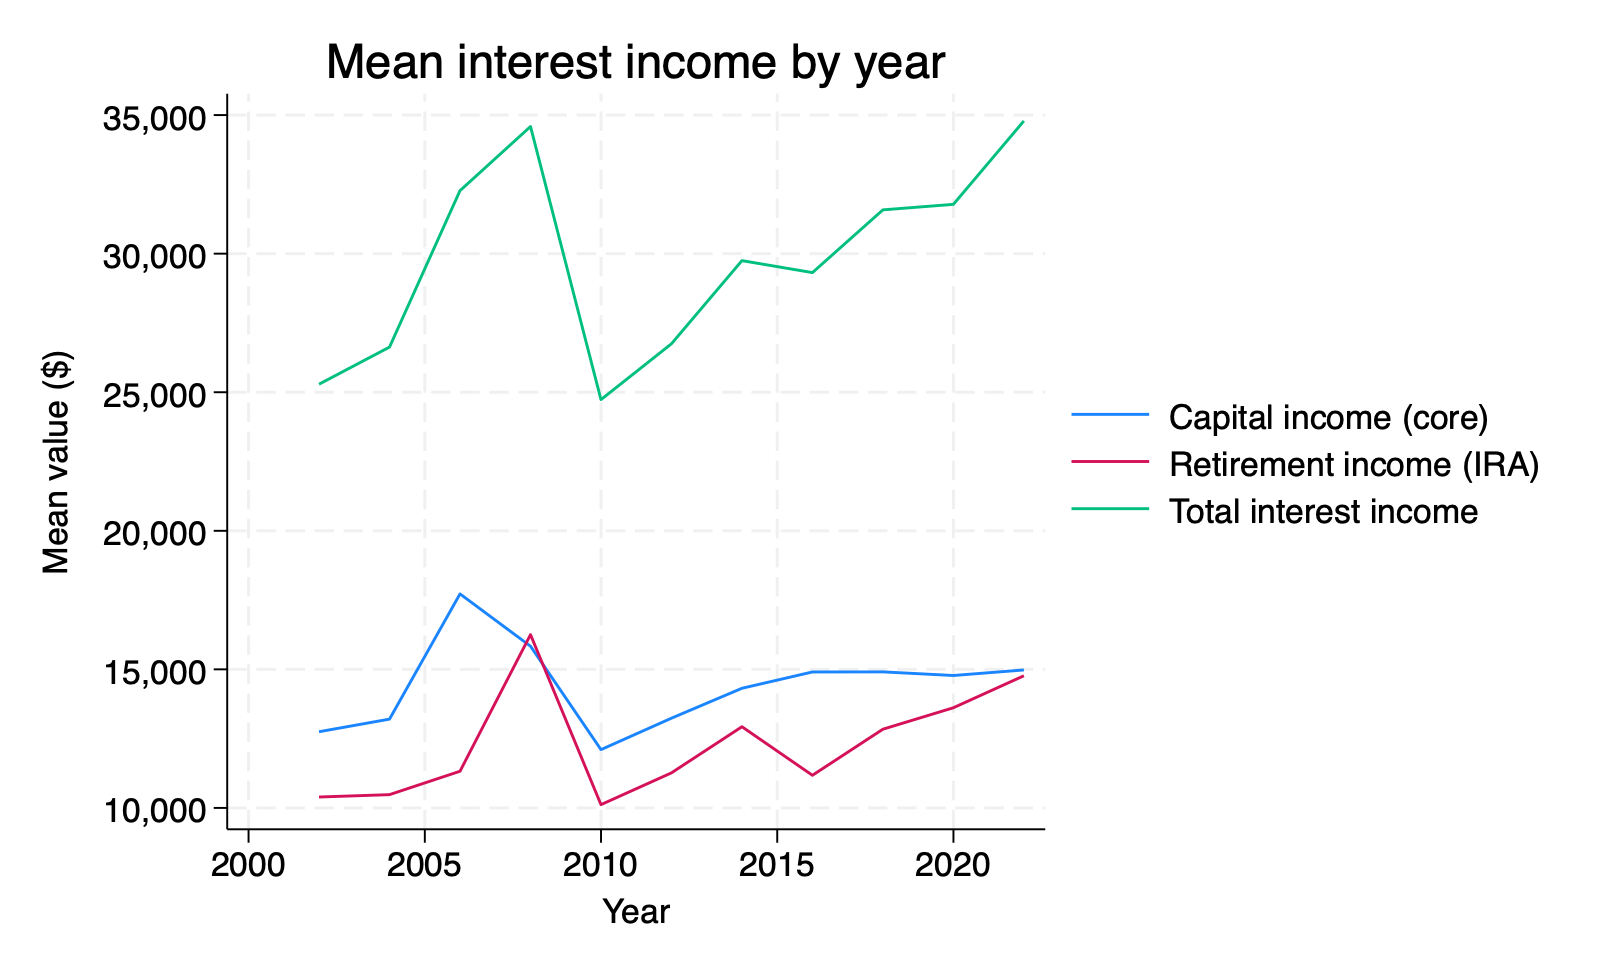
\includegraphics[width=0.8\textwidth]{../../Code/Descriptive/Figures/interest_income_mean_by_year.png}
\caption{Interest income mean by year}
\end{figure}
\FloatBarrier

\subsubsection{Capital gains}

\par The possible asset classes for which capital gains can be computed in the HRS are i) primary residences, ii) secondary residences, iii) other real estate, iv) private business, v) IRA/Keogh (or \say{retirement}), vi) stocks/mutual funds, vii) bonds, viii) checking/savings/money market, ix) cds/t-bills, x) vehicles, xi) other assets. The possible liabilities are i) mortgages on primary residence, ii) mortgage on secondary residence, iii) other home loans, and iv) total other debt.  

\par Capital gains for each asset class are computed as the estimated change in valuation across survey waves. The general trend is that these changes move substantially over time. In the panel (Figure~\ref{fig:cg_core_assets_panels}), business, stocks, and other real estate all show large cyclical swings and end the sample at levels above where they begin, while safe assets (bonds + checking/savings + CDs/T-bills) are flatter and lower-volatility by comparison.

\begin{figure}[H]
\centering
\begin{minipage}[t]{0.48\textwidth}
\centering
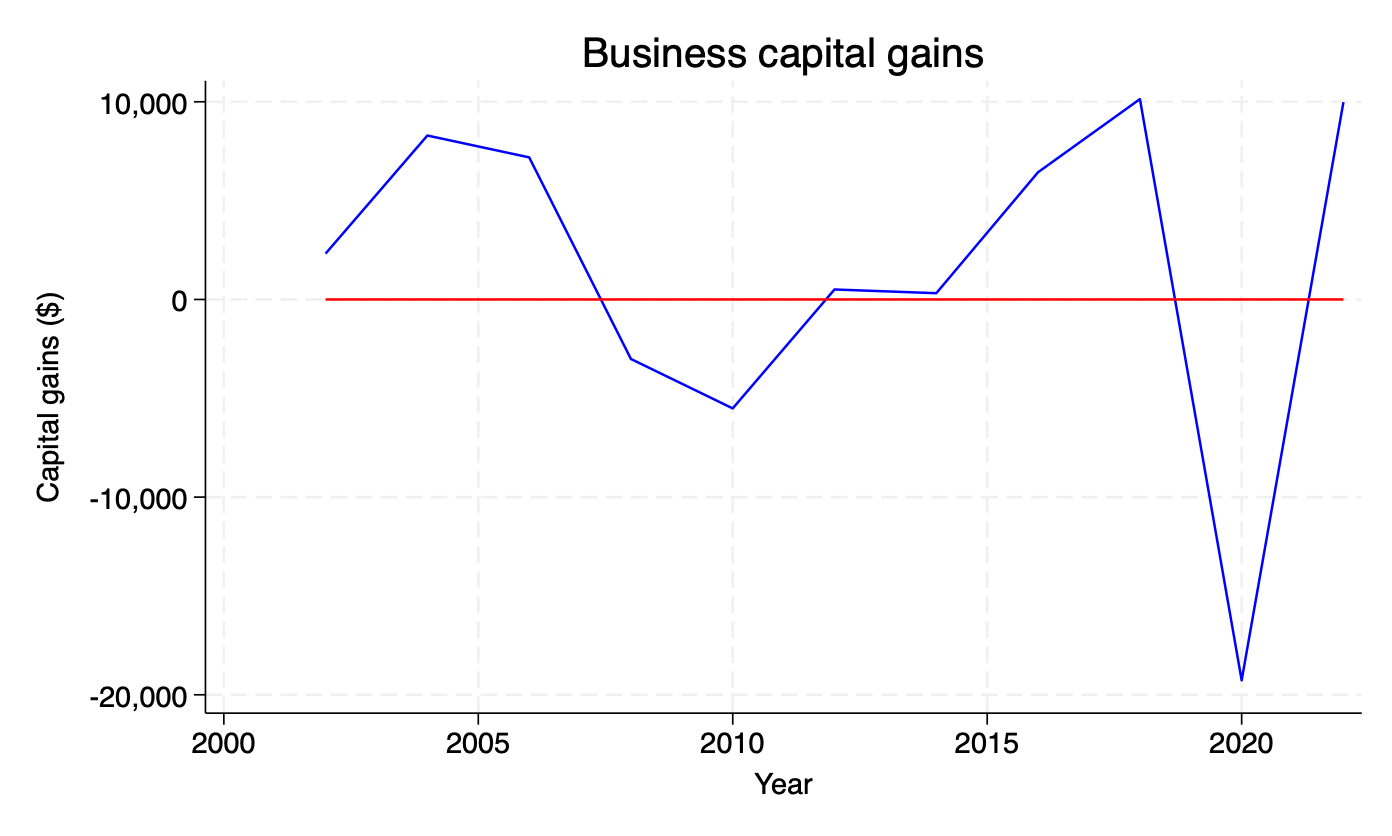
\includegraphics[width=\textwidth]{../../Code/Descriptive/Figures/cg_bus_mean_median_by_year.png}
\end{minipage}\hfill
\begin{minipage}[t]{0.48\textwidth}
\centering
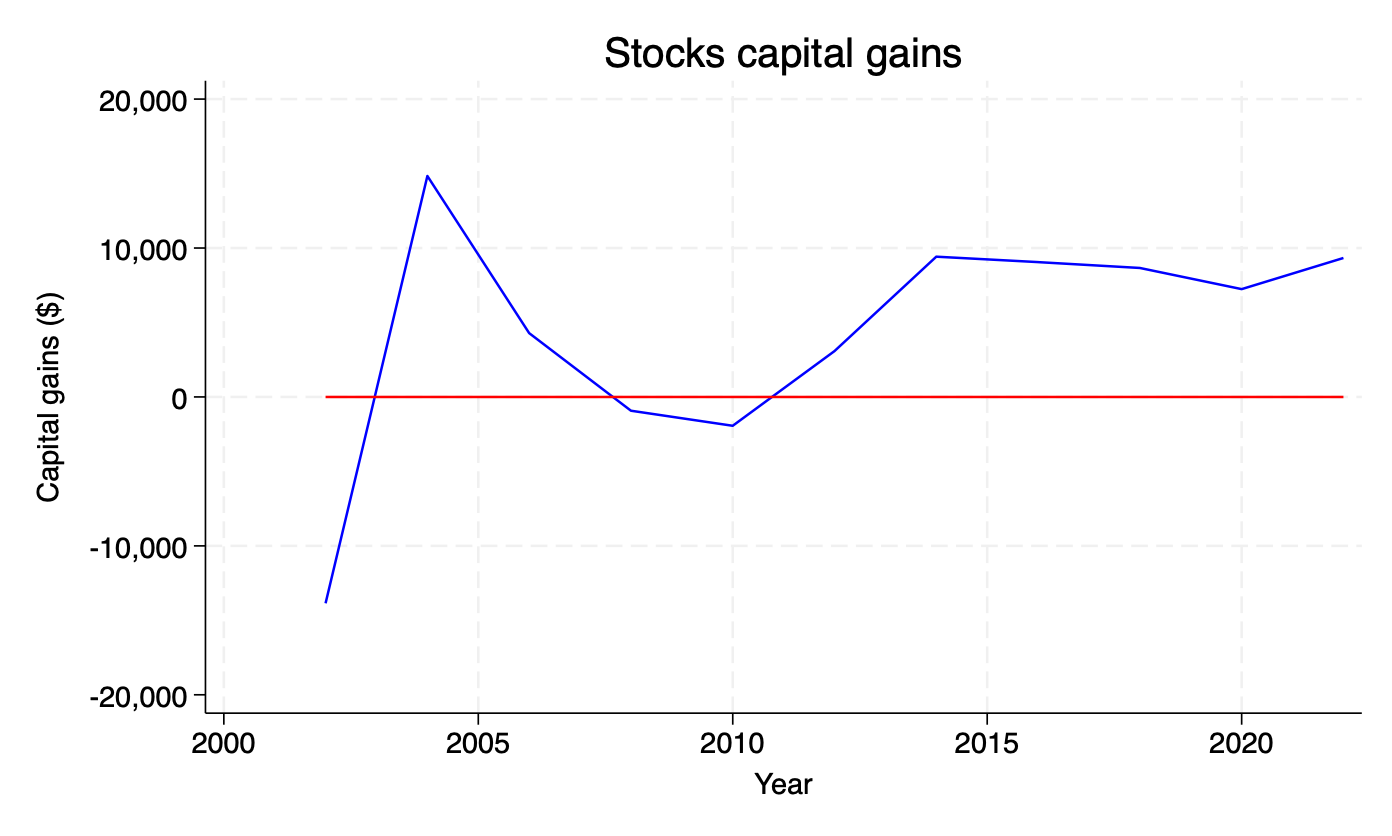
\includegraphics[width=\textwidth]{../../Code/Descriptive/Figures/cg_stk_mean_median_by_year.png}
\end{minipage}

\vspace{0.6em}
\begin{minipage}[t]{0.48\textwidth}
\centering
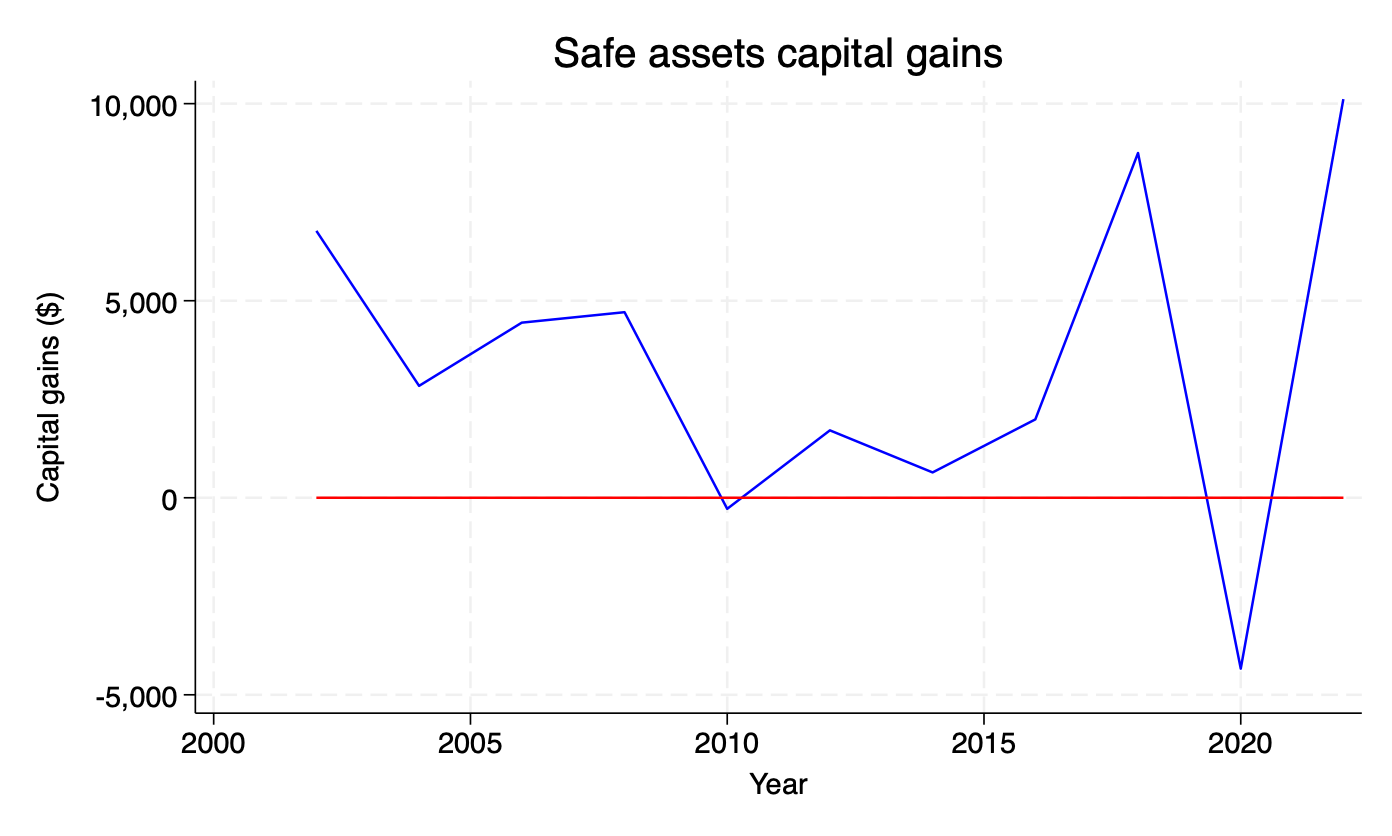
\includegraphics[width=\textwidth]{../../Code/Descriptive/Figures/cg_safe_mean_median_by_year.png}
\end{minipage}\hfill
\begin{minipage}[t]{0.48\textwidth}
\centering
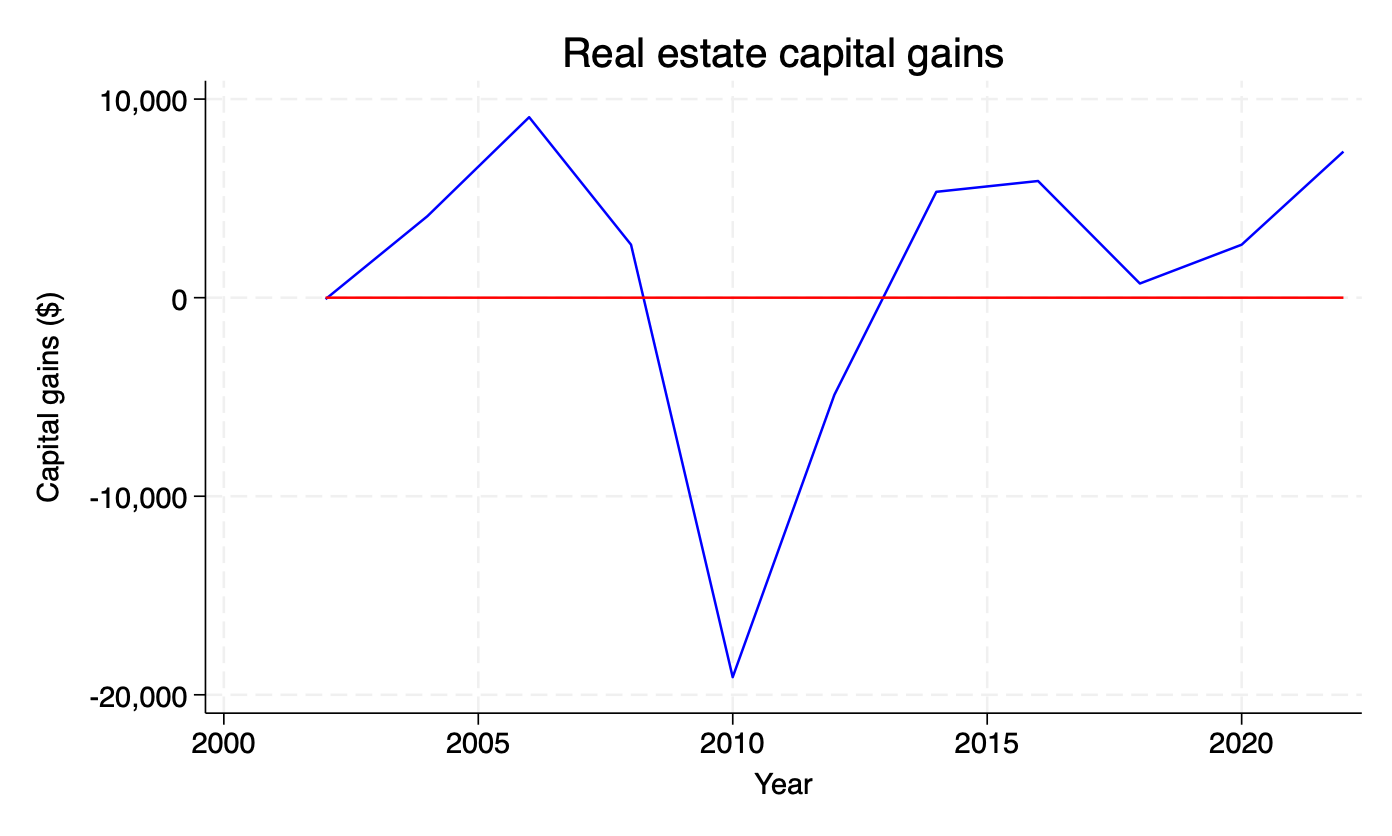
\includegraphics[width=\textwidth]{../../Code/Descriptive/Figures/cg_re_mean_median_by_year.png}
\end{minipage}
\caption{Capital gains in core assets, by year}
\label{fig:cg_core_assets_panels}
\end{figure}
\FloatBarrier

\begin{figure}[H]
\centering
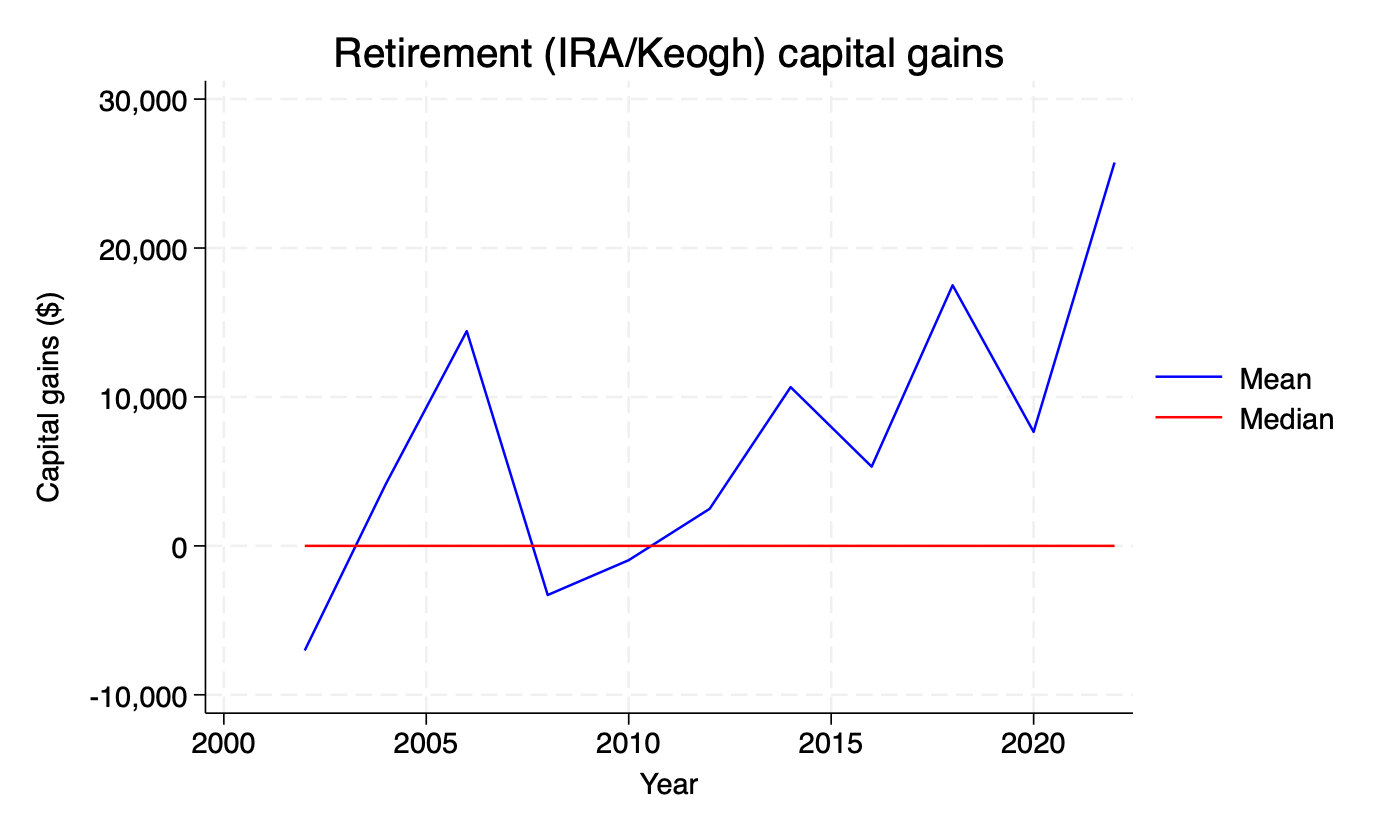
\includegraphics[width=0.8\textwidth]{../../Code/Descriptive/Figures/cg_ira_mean_median_by_year.png}
\caption{Capital gains in retirement assets, by year}
\label{fig:cg_ira_by_year}
\end{figure}
\FloatBarrier

\par Another feature that is apparent by taking a look at capital gains is that, most respondent hold no assets in a particular class. This can be seen by the red median line at $0$ for most waves. In the residential panel (Figure~\ref{fig:cg_residential_panels}), the primary-residence series is much larger in level and volatility than the secondary-residence series, and only primary residence shows a clearly positive median in some years. This is another sign that the data is sensible so far -- large amount of non-participation despite evidence of returns is consistent with the empirically documented equity premium puzzle.

\begin{figure}[H]
\centering
\begin{minipage}[t]{0.48\textwidth}
\centering
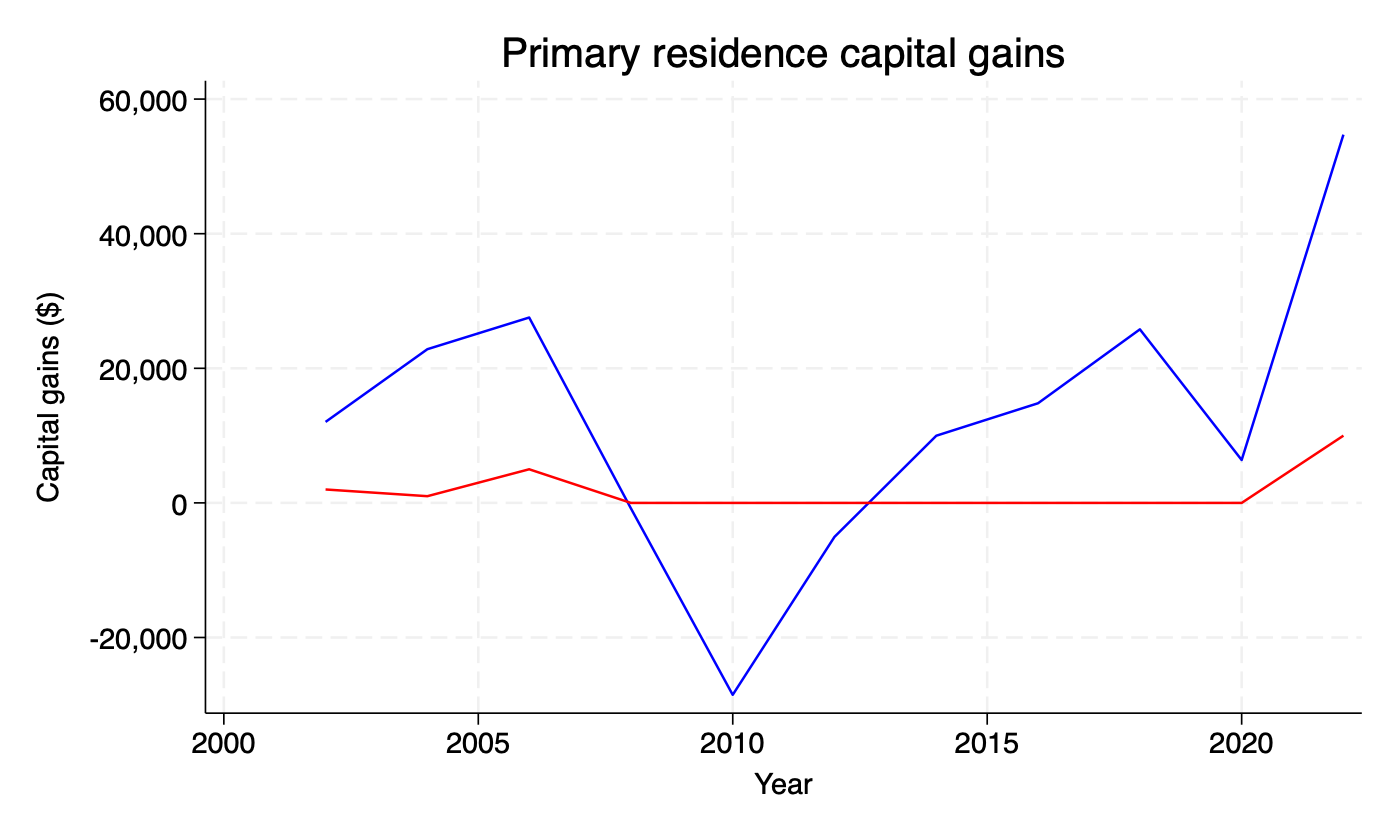
\includegraphics[width=\textwidth]{../../Code/Descriptive/Figures/cg_res_mean_median_by_year.png}
\end{minipage}\hfill
\begin{minipage}[t]{0.48\textwidth}
\centering
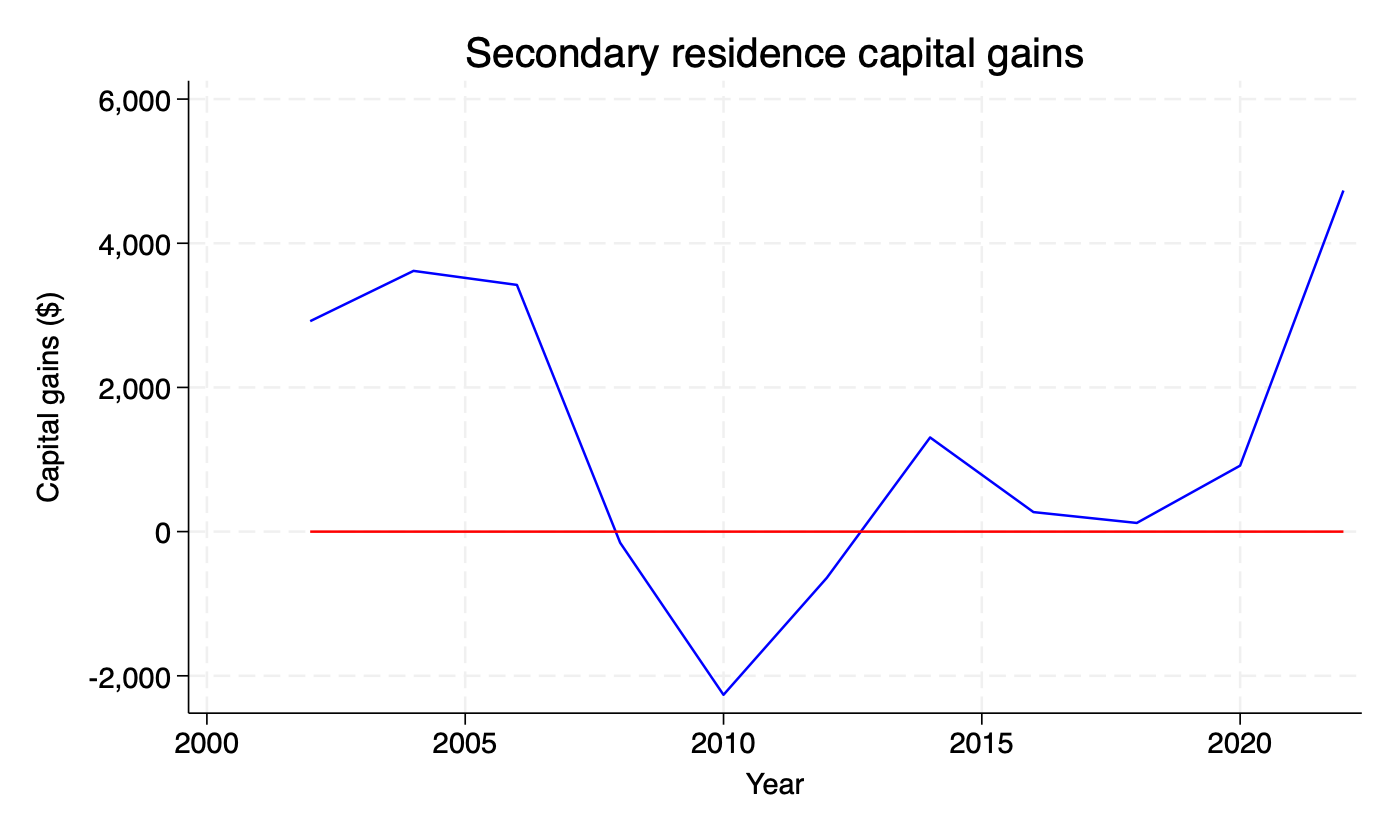
\includegraphics[width=\textwidth]{../../Code/Descriptive/Figures/cg_res2_mean_median_by_year.png}
\end{minipage}
\caption{Capital gains in residential assets, by year}
\label{fig:cg_residential_panels}
\end{figure}
\FloatBarrier

\par Notably, the synchronized dip around 2008--2010 for primary residence, secondary residence, and other real estate is also a good sign regarding how reliably measured the data is.

%%%%%%%

\subsubsection{Net investment flows}

\par Net investment flows are vital in computing returns accurately because capital gains and interest income can miss other flows of value into a given asset class. In the HRS dataset, net investment flows are the only variable relevant to the returns calculation that RAND did not clean and process. For this reason, there are substantially less observation for this variable per asset class than the others. To work around this, I do two things. First, I process the net investment flow per asset class myself by using the associated flag variable (asking yes or no if an individual has \say{bought or sold since the previous wave}) for each variable. Second, I assume that if an individual receives interest income on that asset class, but their flow in nonmissing, then the nonmissing flow to that asset class is treated as 0.\footnote{Non-missing interest income (and capital gains) indicate participation within an asset class.}

\par With this in mind, I present a figure of net investment flows into the assets available in the dataset. As you can see, the magnitudes for flows into a given class are comparable. I use these flows to construct net investment flows into i) \textbf{core assets}, ii) \textbf{retirement assets}, iii) \textbf{residential assets}, iv) \textbf{core and residential assets}, and v) \textbf{net wealth}.

\begin{figure}[H]
\centering
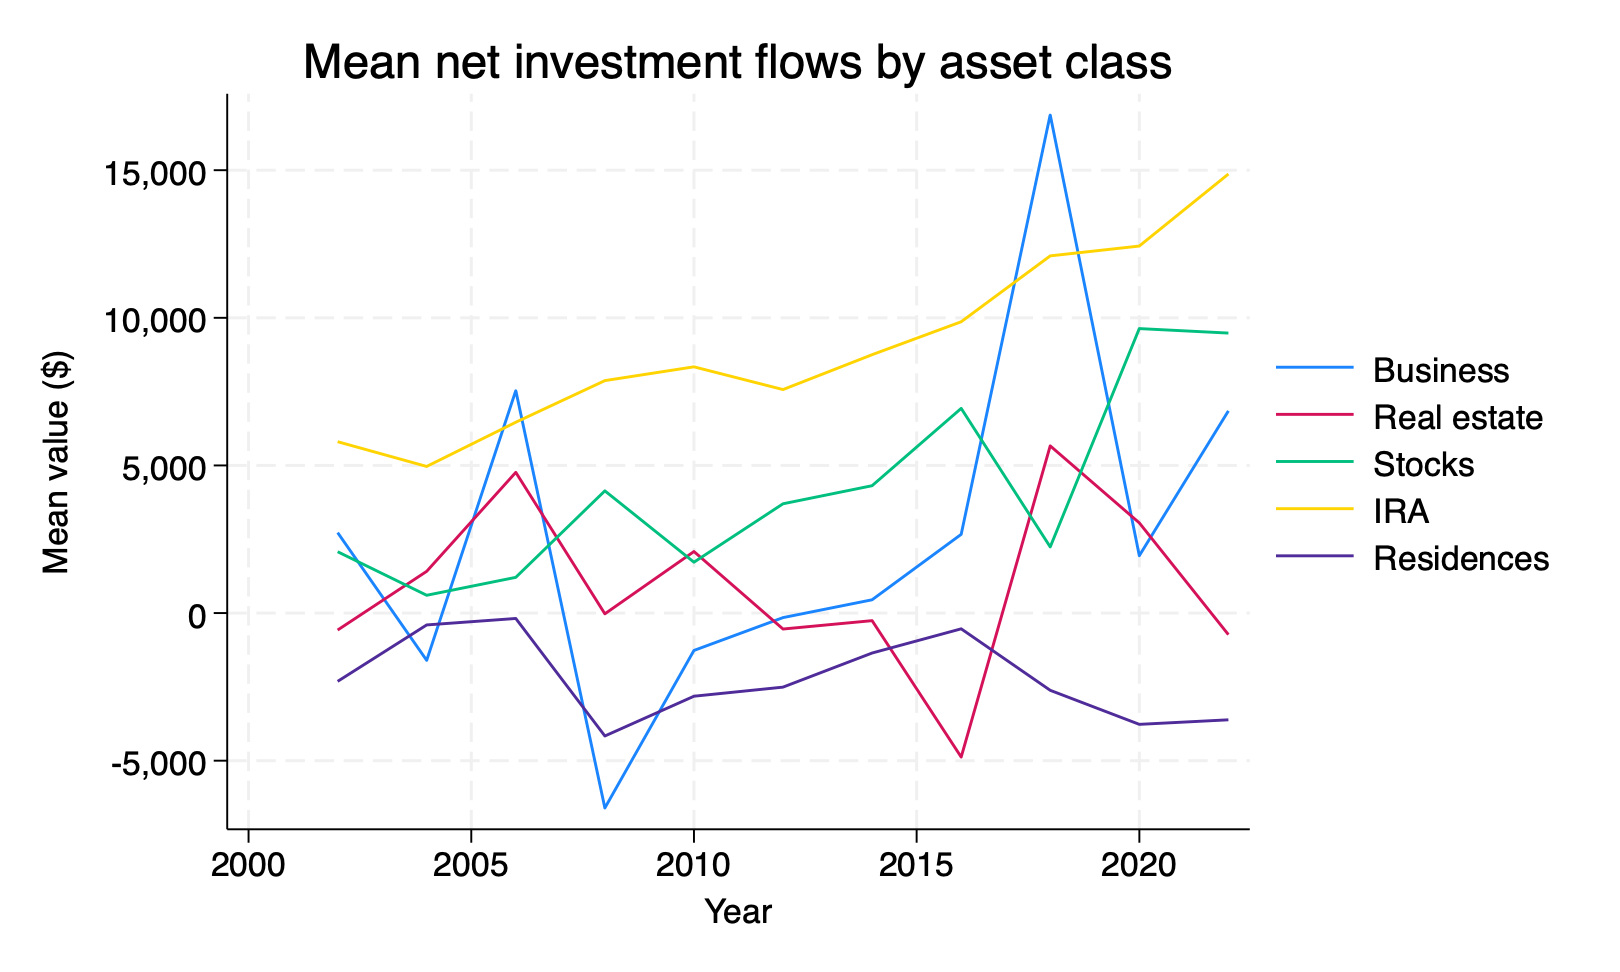
\includegraphics[width=0.8\textwidth]{../../Code/Descriptive/Figures/flows_by_asset_mean_by_year.png}
\caption{Flows by asset, mean by year}
\end{figure}
\FloatBarrier

\subsubsection{Wealth and inequality}

\par After defining asset classes, I consider mean wealth within these narrowly defined asset classes for each year of the sample. Interestingly, retirement assets seem to perform the worst in terms of average returns. Core assets seem to offer the best performance, and all asset classes see a downward dive leading up to 2010 -- historically accurate in the context of investment performance during the global financial crisis.

\begin{figure}[H]
\centering
\begin{minipage}[t]{0.48\textwidth}
\centering
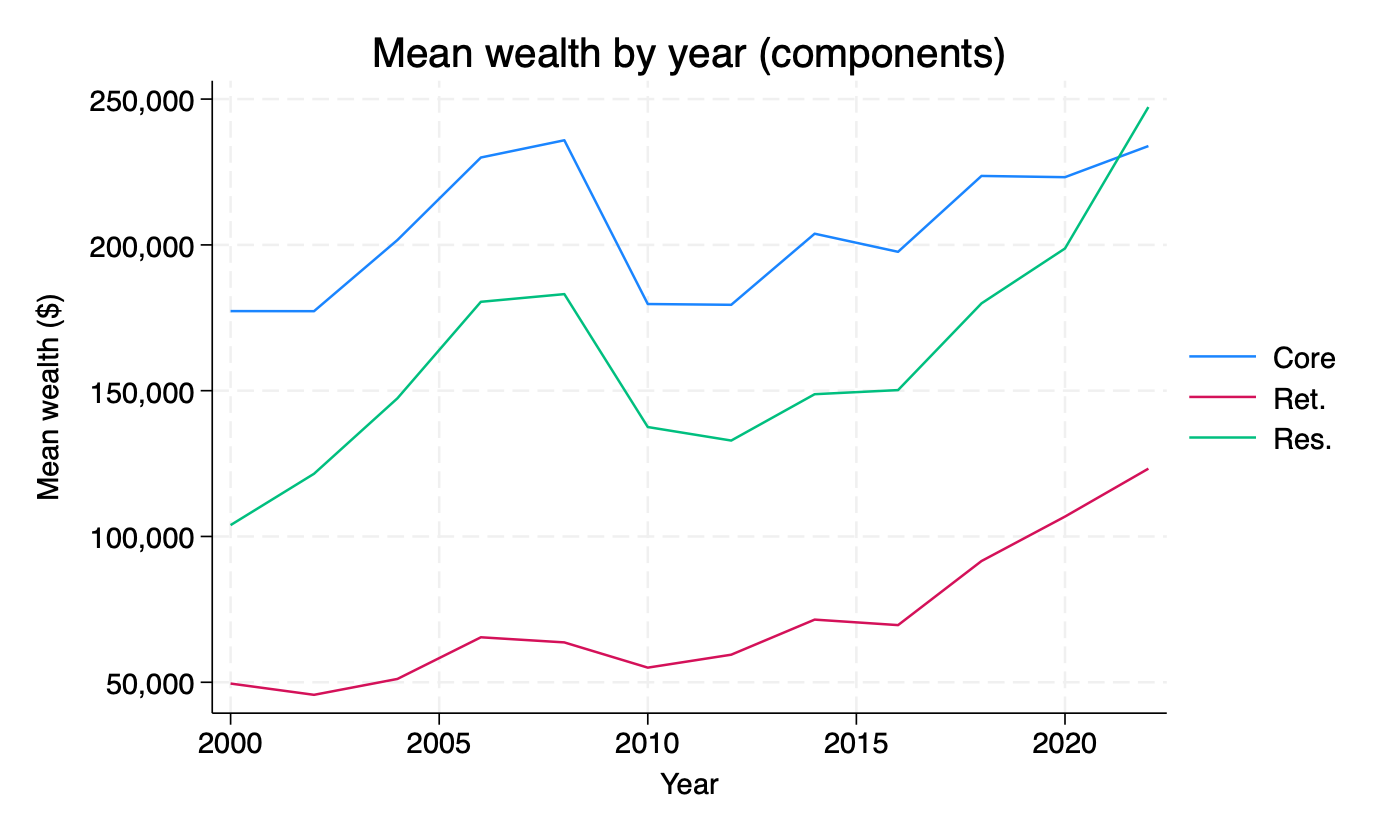
\includegraphics[width=\textwidth]{../../Code/Descriptive/Figures/wealth_mean_by_year_components.png}
\end{minipage}\hfill
\begin{minipage}[t]{0.48\textwidth}
\centering
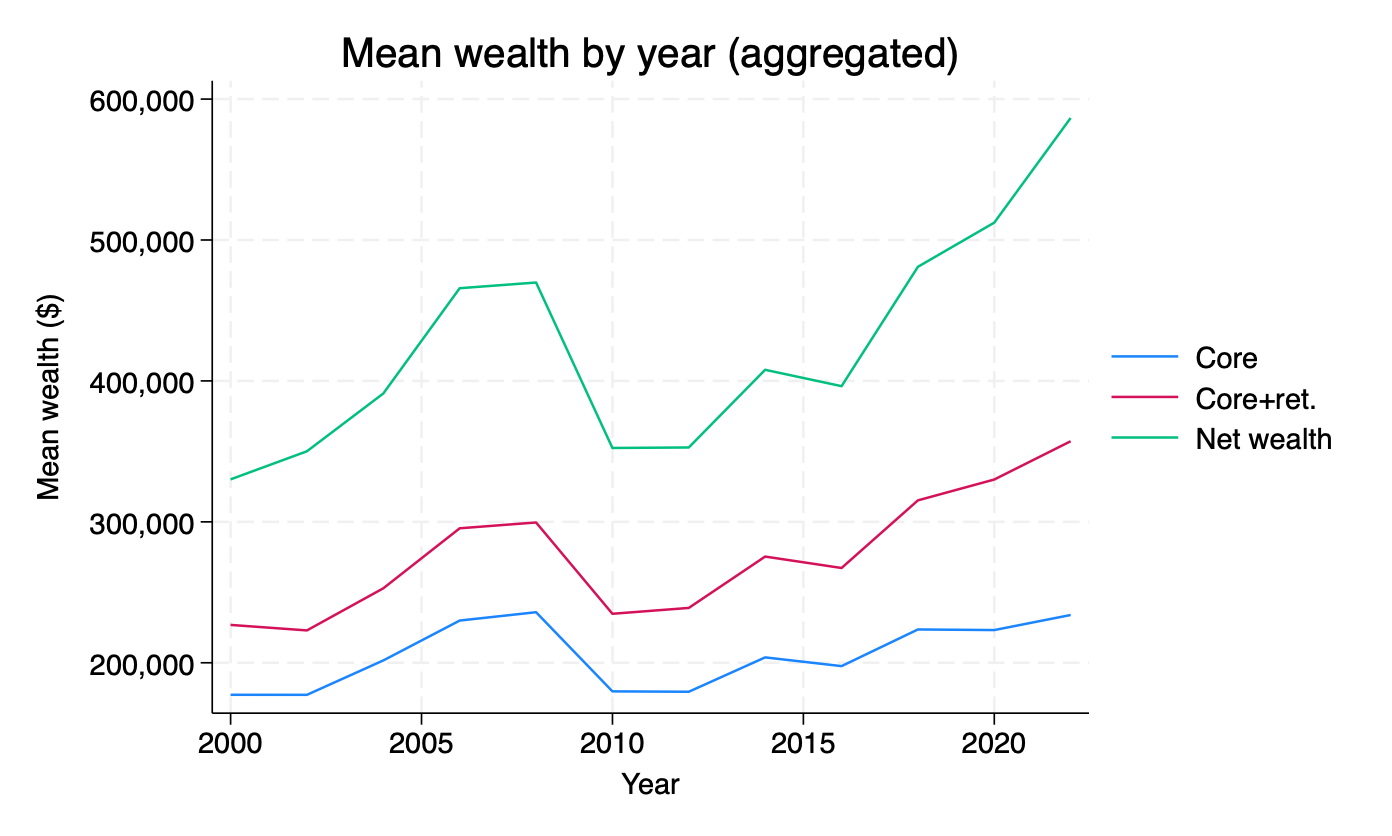
\includegraphics[width=\textwidth]{../../Code/Descriptive/Figures/wealth_mean_by_year_agg.png}
\end{minipage}
\caption{Mean wealth by year}
\label{fig:wealth_mean_by_year_panels}
\end{figure}
\FloatBarrier

\par I turn attention to measures of wealth in the sample based on the portfolio definitions: i) net wealth in core assets, ii) net wealth in core and retirement assets, iii) total net wealth.

\par I consider the distribution of these measures of income and wealth across respondents of the survey in the following figures. For income, the measure of labor income is significantly more unequally distributed than the measure of total income in the sample. This is likely an artifact of the sampling method of the HRS (older likely overrepresented and are towards the end of their working years).

\begin{figure}[H]
\centering
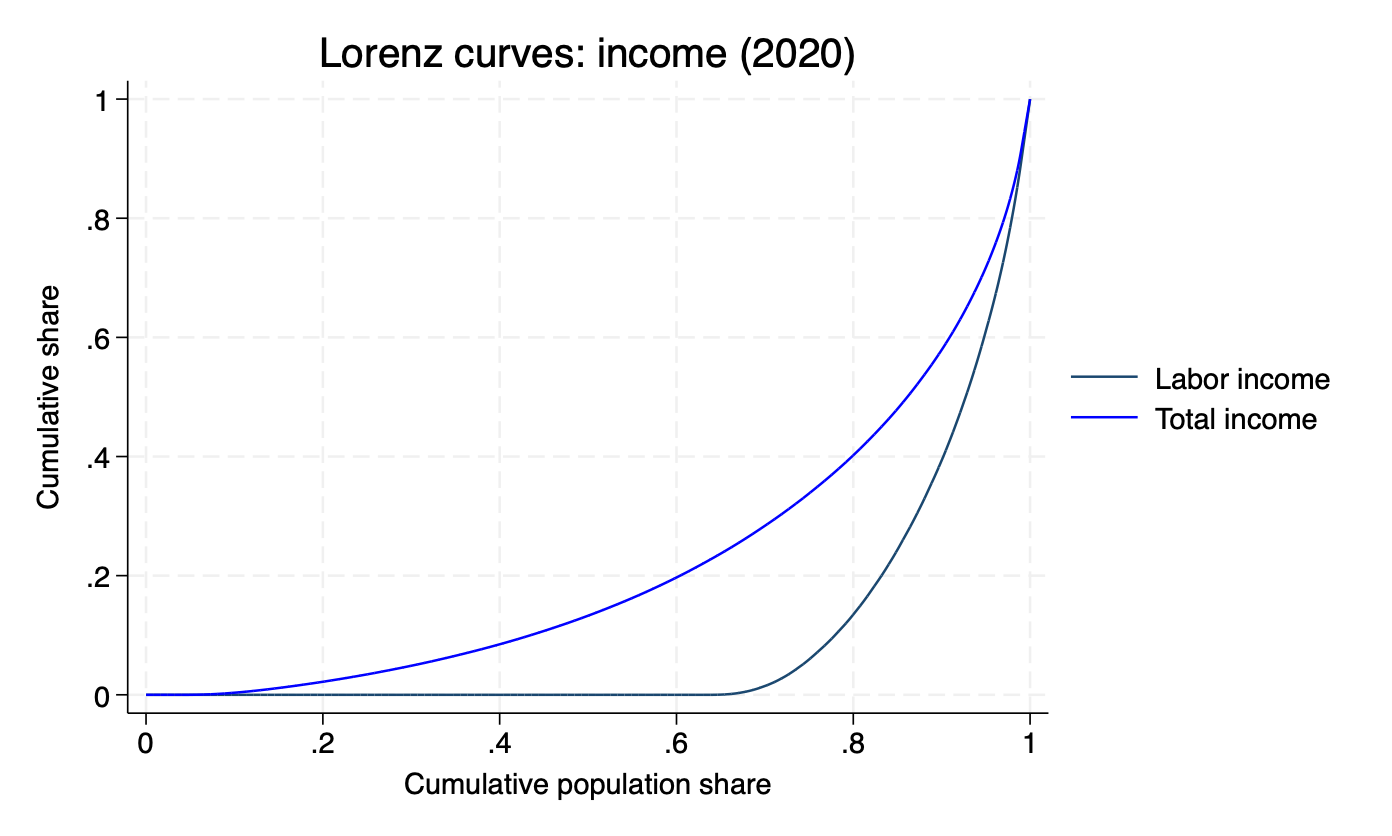
\includegraphics[width=0.8\textwidth]{../../Code/Descriptive/Figures/lorenz_income_2020.png}
\caption{Lorenz: income (2020)}
\label{fig:lorenz_income_2020}
\end{figure}
\FloatBarrier

\begin{figure}[H]
\centering
\begin{minipage}[t]{0.48\textwidth}
\centering
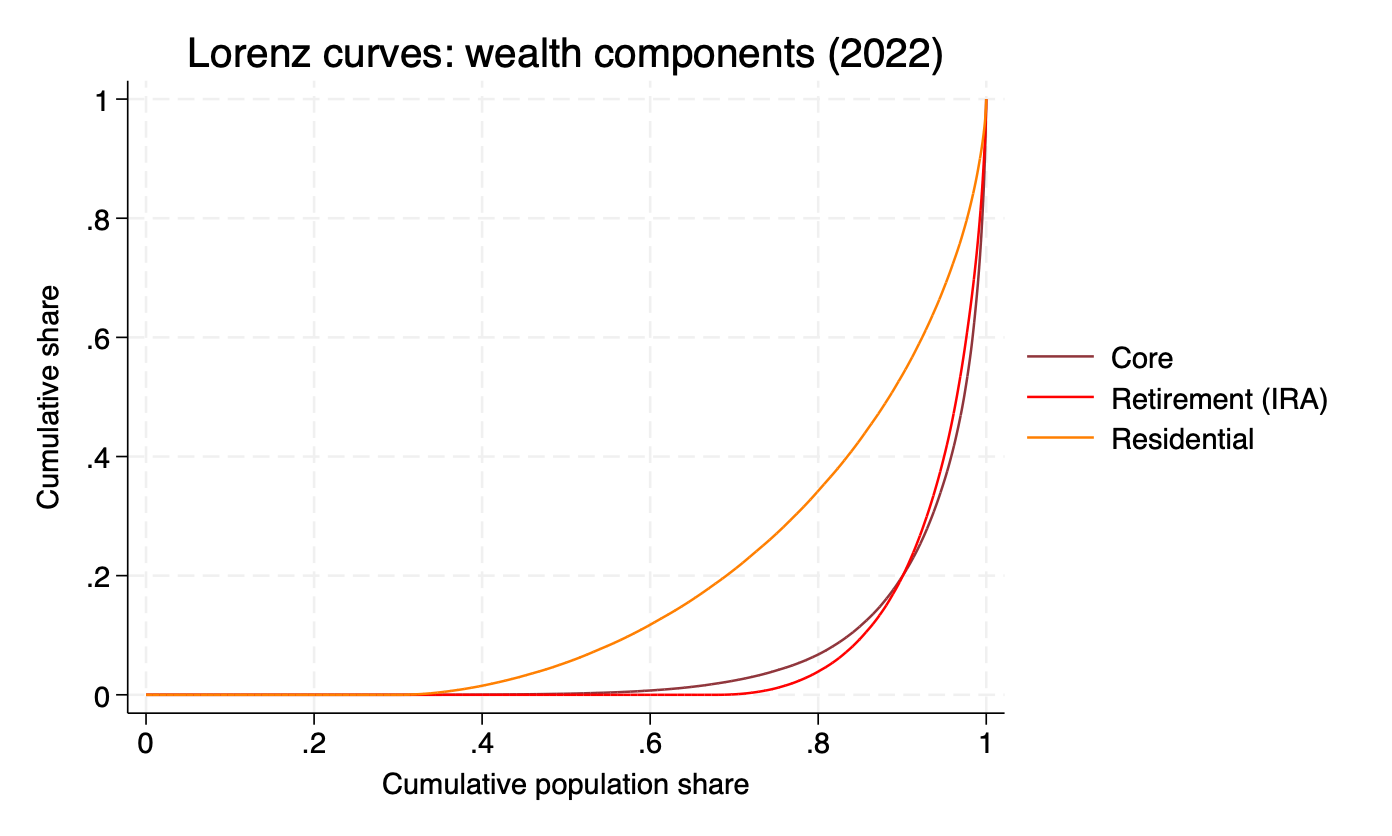
\includegraphics[width=\textwidth]{../../Code/Descriptive/Figures/lorenz_wealth_components_2022.png}
\end{minipage}\hfill
\begin{minipage}[t]{0.48\textwidth}
\centering
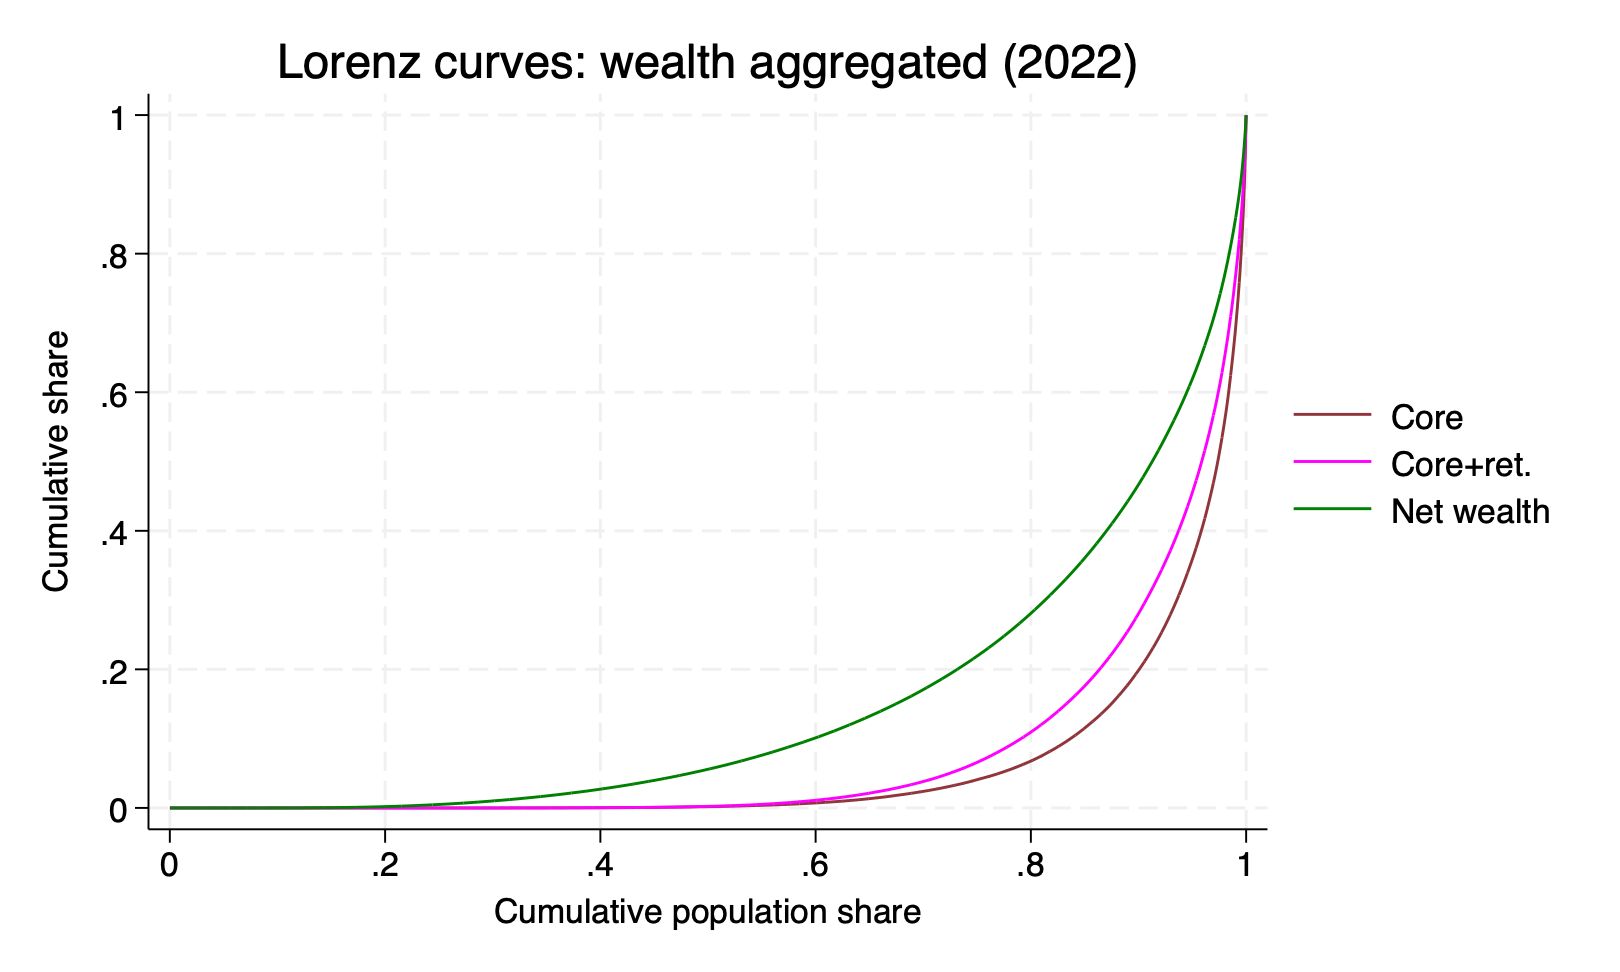
\includegraphics[width=\textwidth]{../../Code/Descriptive/Figures/lorenz_wealth_agg_2022.png}
\end{minipage}
\caption{Lorenz: wealth (2022)}
\label{fig:lorenz_wealth_panels_2022}
\end{figure}
\FloatBarrier

\par For wealth, holdings in core assets and retirement assets are more unequally distributed than holdings in residential assets. This is in line with common knowledge that home ownership is the most common form of asset ownership in the U.S.

\par Interestingly, the distribution of net wealth become less unequal when it is extended to incorporate retirement assets on top of core assets. this can be seen in the following figure .

\subsubsection{Portfolio composition}

\par To describe the composition of portfolio during the period, I document mean portfolio shares for the relevant asset classes.

\begin{figure}[H]
\centering
\begin{minipage}[t]{0.48\textwidth}
\centering
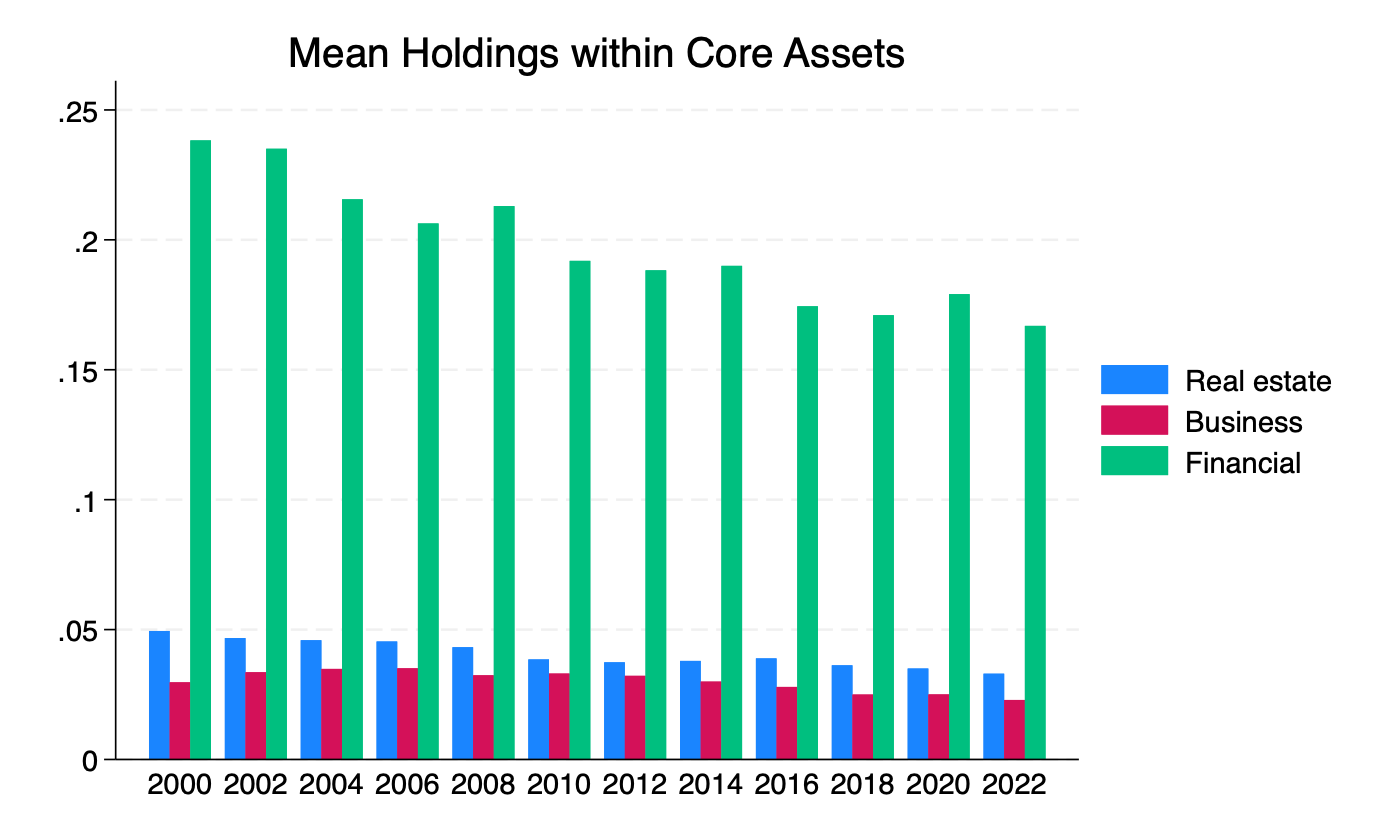
\includegraphics[width=\textwidth]{../../Code/Descriptive/Figures/share_mean_by_year_core_components.png}
\end{minipage}\hfill
\begin{minipage}[t]{0.48\textwidth}
\centering
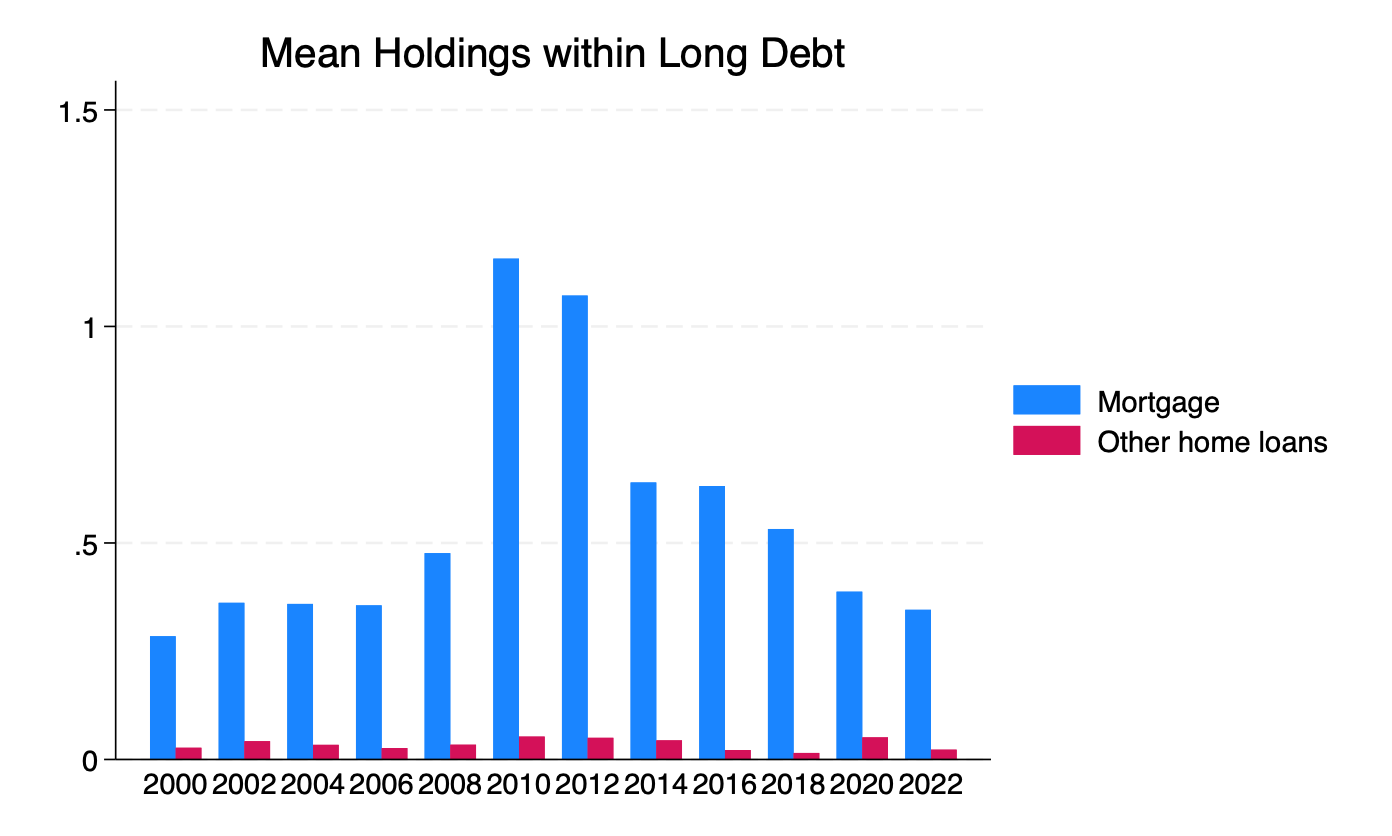
\includegraphics[width=\textwidth]{../../Code/Descriptive/Figures/share_mean_by_year_debt_long_components.png}
\end{minipage}
\caption{Mean holdings within assets and liabilities, by year}
\label{fig:share_holdings_assets_liabilities}
\end{figure}
\FloatBarrier

\begin{figure}[H]
\centering
\begin{minipage}[t]{0.48\textwidth}
\centering
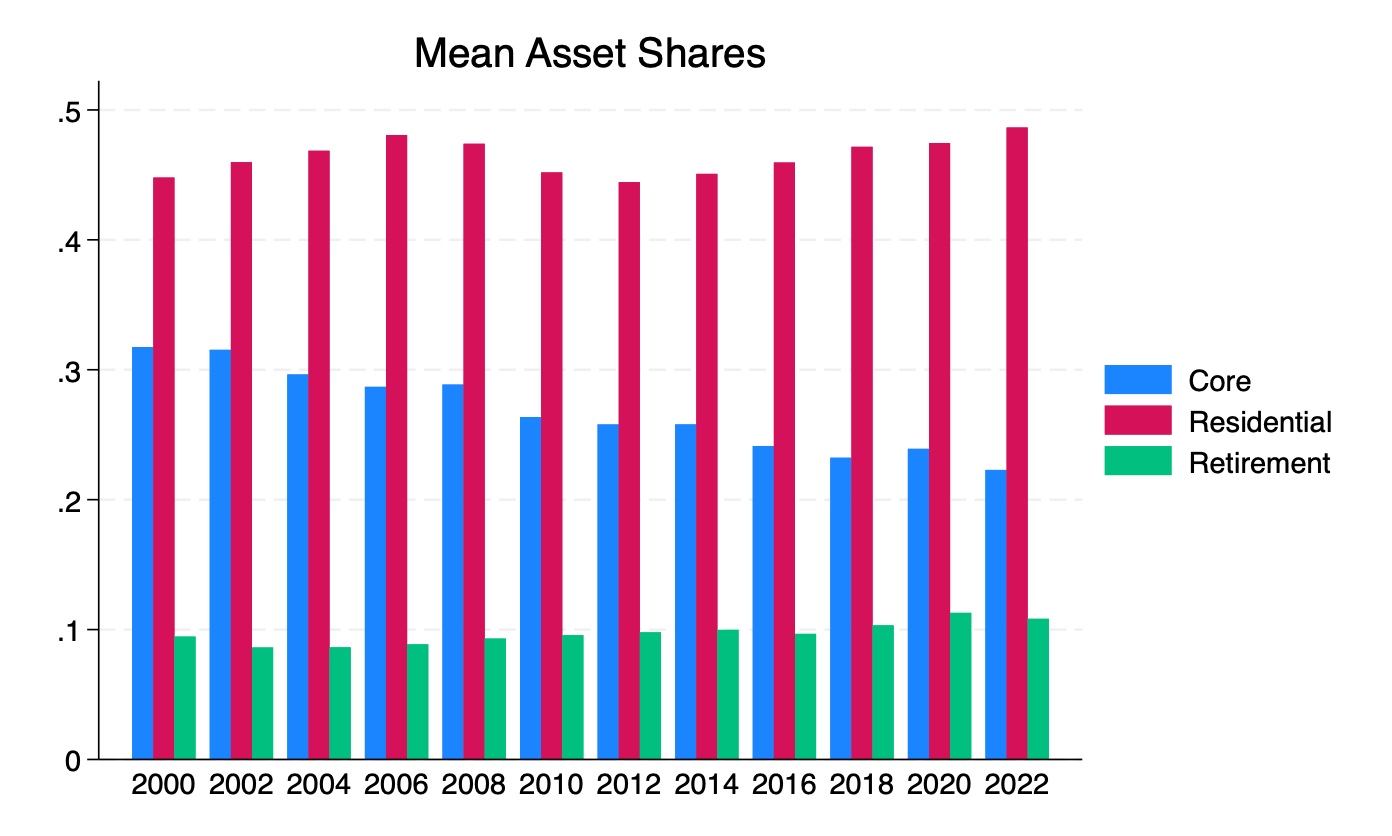
\includegraphics[width=\textwidth]{../../Code/Descriptive/Figures/share_mean_by_year_core_res_ret.png}
\end{minipage}\hfill
\begin{minipage}[t]{0.48\textwidth}
\centering
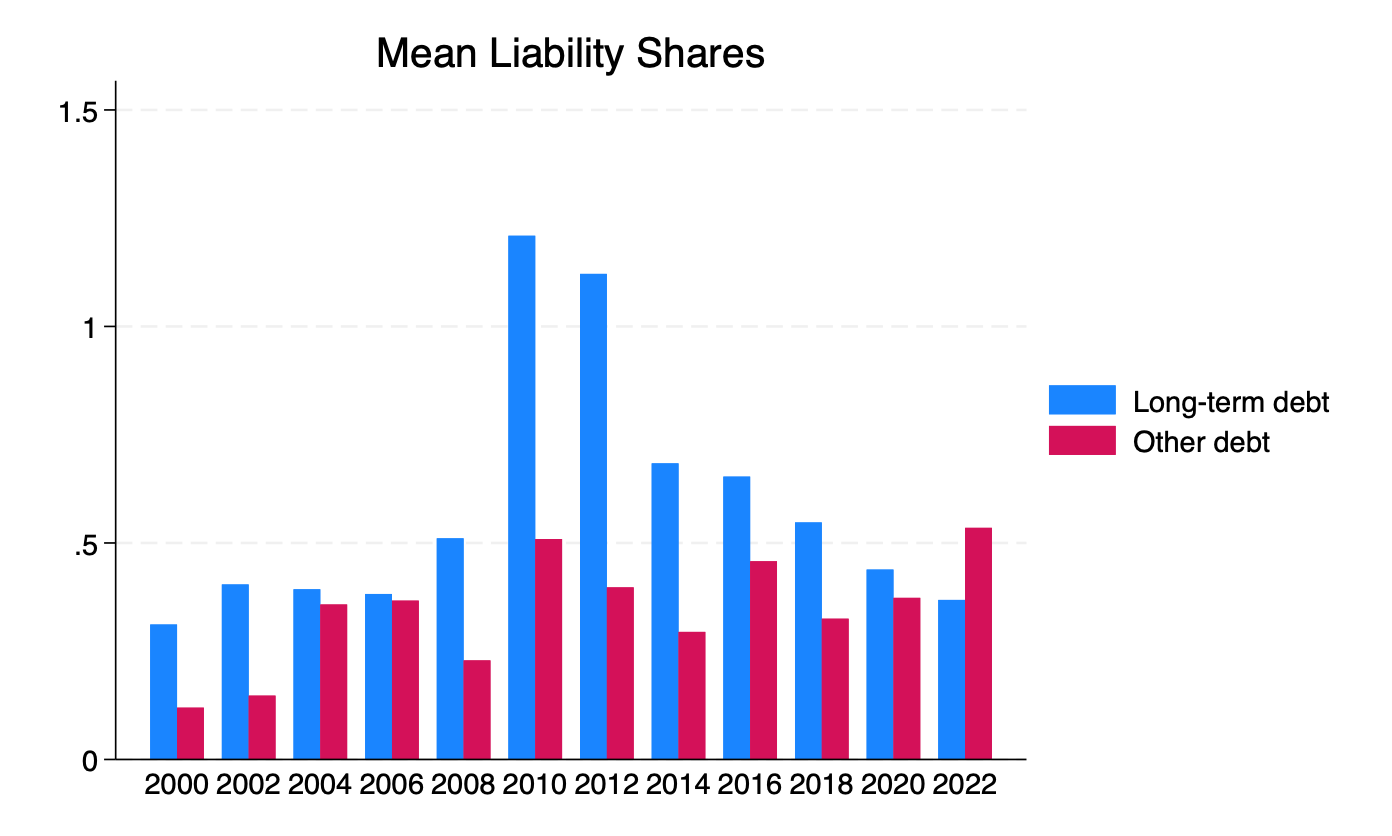
\includegraphics[width=\textwidth]{../../Code/Descriptive/Figures/share_mean_by_year_debt_long_other.png}
\end{minipage}
\caption{Mean asset and debt shares, by year}
\label{fig:share_assets_debt_year}
\end{figure}
\FloatBarrier

\par Investment behavior is likely to vary with income and wealth. Asset shares (core, residential, retirement) by percentile of labor income, total income, and net wealth (2020): 

\begin{figure}[H]
\centering
\begin{minipage}[t]{0.48\textwidth}
\centering
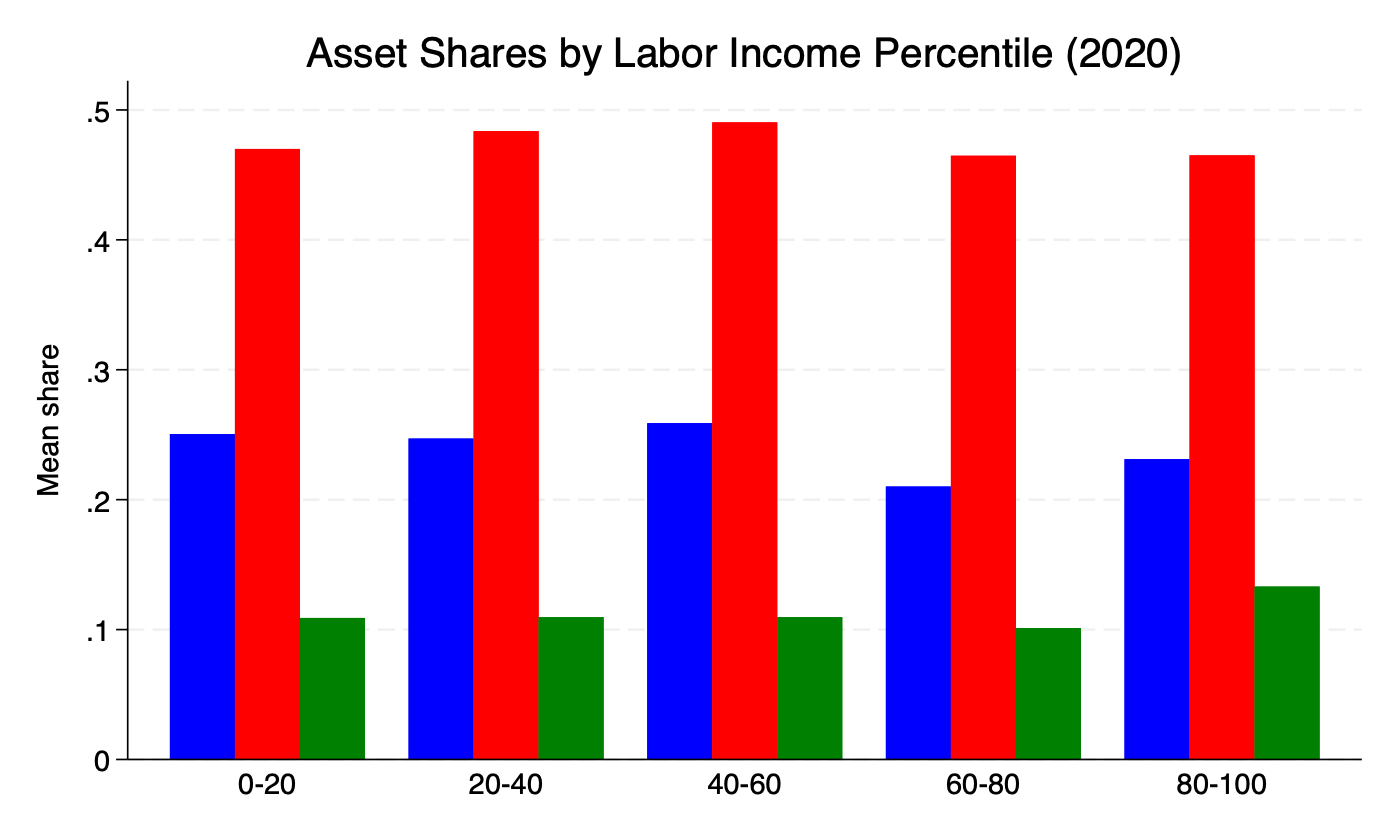
\includegraphics[width=\textwidth]{../../Code/Descriptive/Figures/asset_shares_by_labor_inc_pct_2020.png}
\end{minipage}\hfill
\begin{minipage}[t]{0.48\textwidth}
\centering
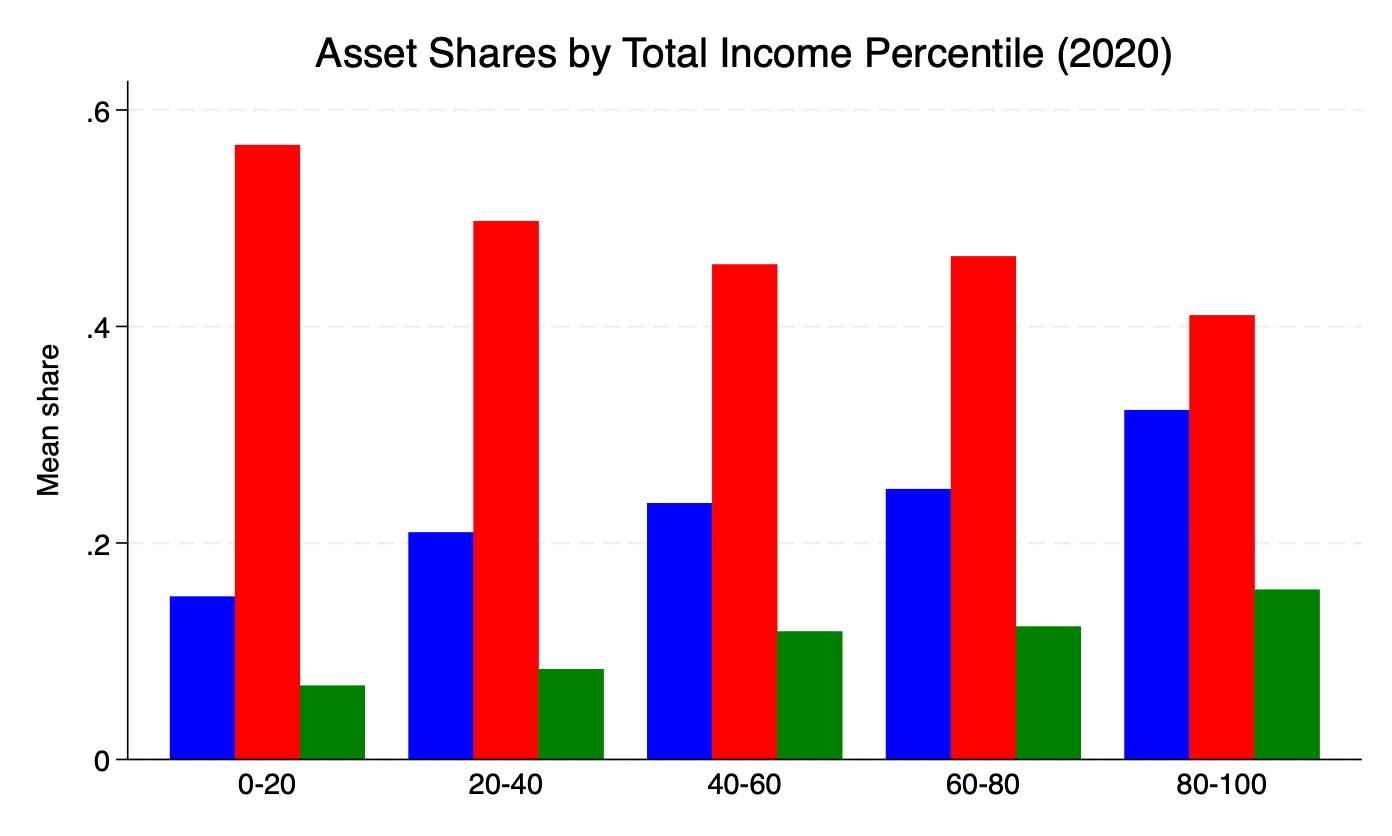
\includegraphics[width=\textwidth]{../../Code/Descriptive/Figures/asset_shares_by_total_inc_pct_2020.png}
\end{minipage}
\caption{Asset shares by labor and total income percentiles (2020)}
\label{fig:asset_shares_income_panels_2022}
\end{figure}
\FloatBarrier


\begin{figure}[H]
\centering
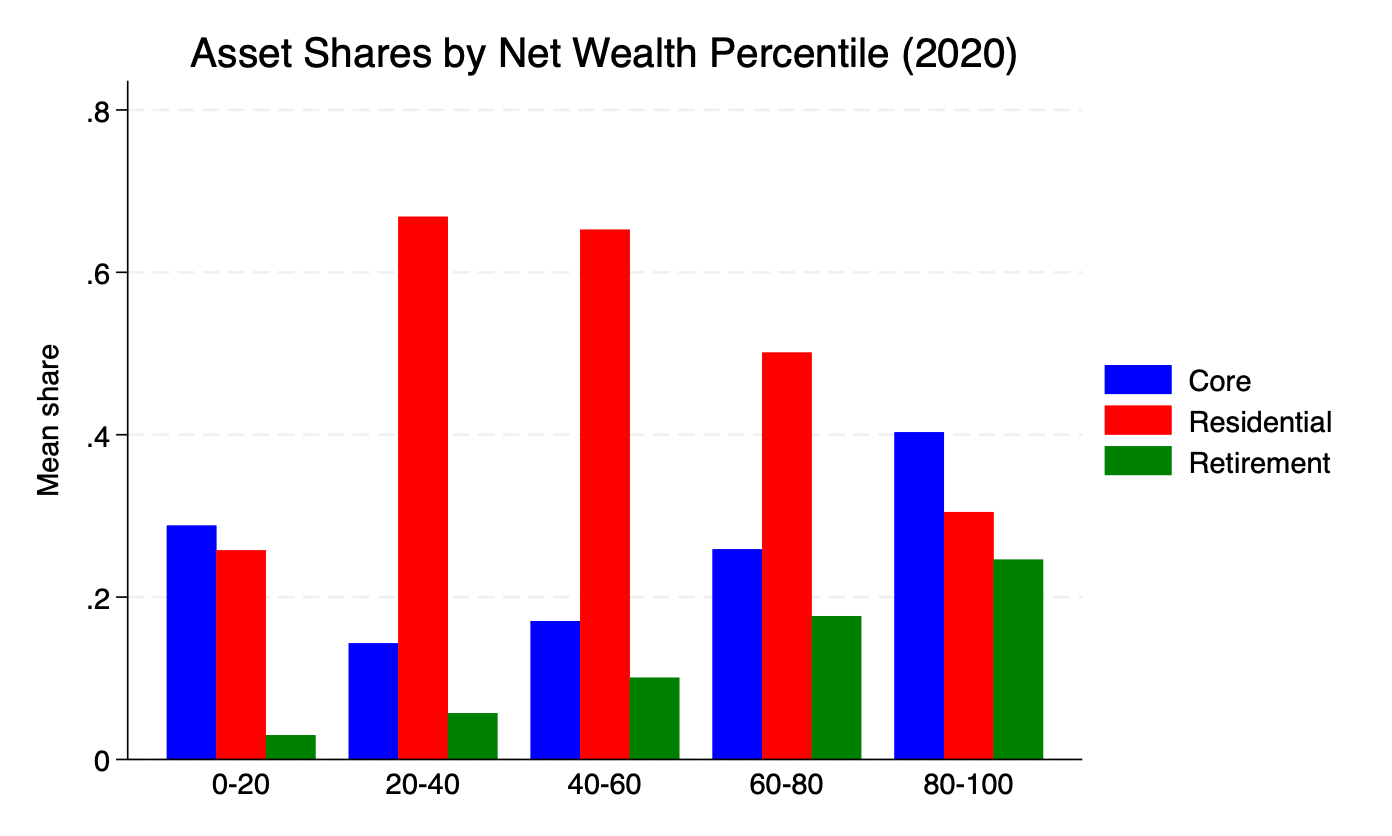
\includegraphics[width=0.8\textwidth]{../../Code/Descriptive/Figures/asset_shares_by_net_pct_2020.png}
\caption{Asset shares by net wealth percentile (2020)}
\end{figure}
\FloatBarrier

\par We can also look at the same breakdown by income and wealth percentiles but for the ratio of debt to gross assets. This is captured in the following figures .

\begin{figure}[H]
\centering
\begin{minipage}[t]{0.48\textwidth}
\centering
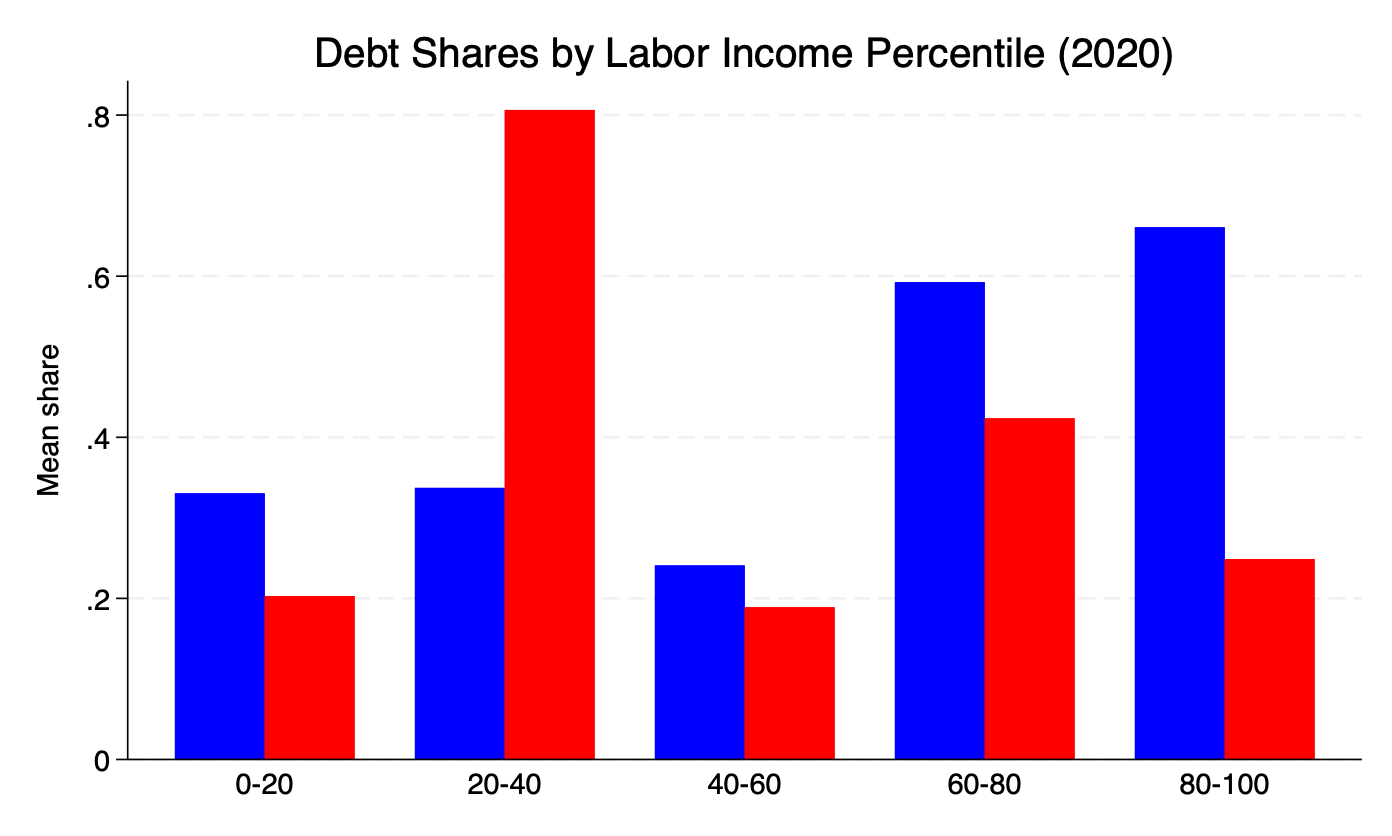
\includegraphics[width=\textwidth]{../../Code/Descriptive/Figures/debt_shares_by_labor_inc_pct_2020.png}
\end{minipage}\hfill
\begin{minipage}[t]{0.48\textwidth}
\centering
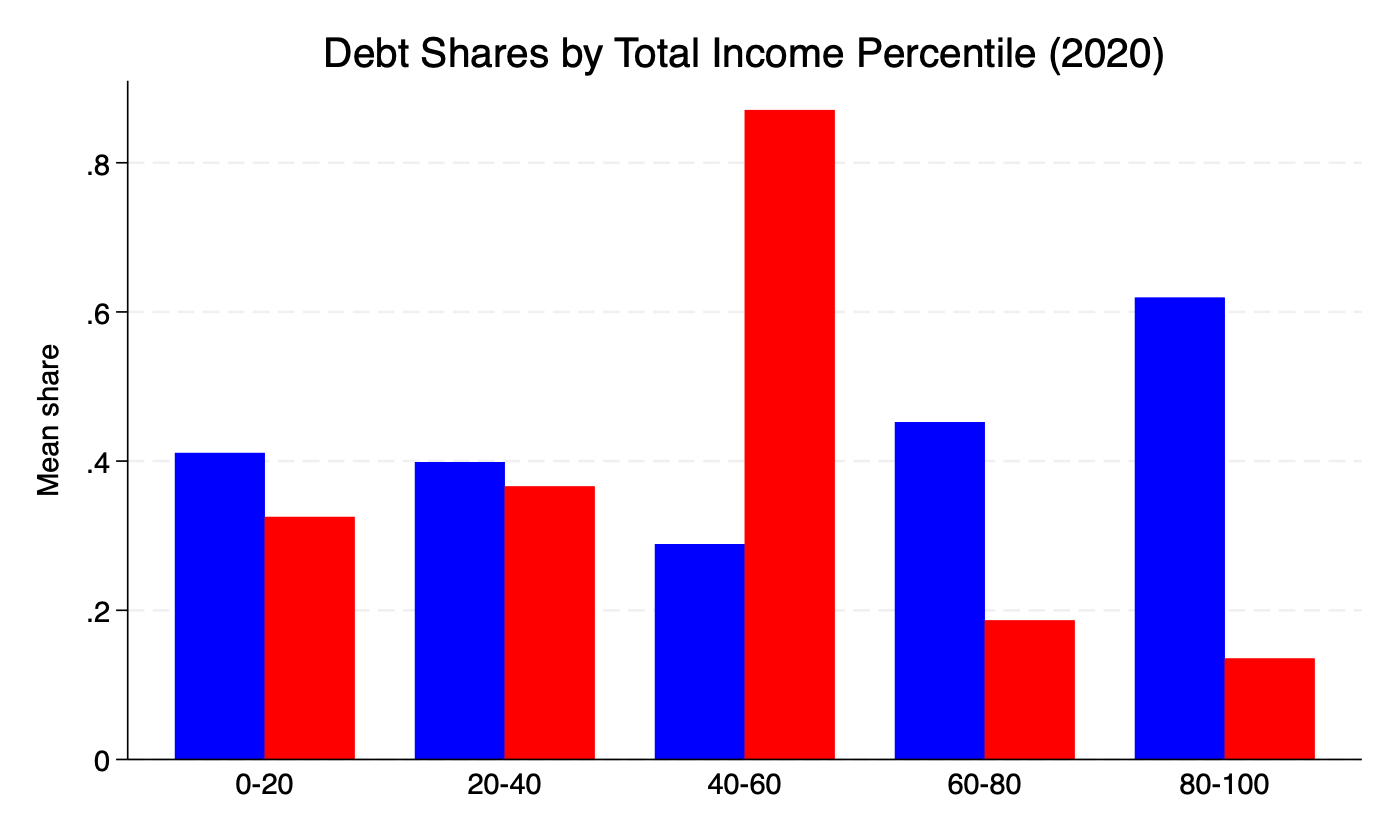
\includegraphics[width=\textwidth]{../../Code/Descriptive/Figures/debt_shares_by_total_inc_pct_2020.png}
\end{minipage}
\caption{Debt shares by labor and total income percentiles (2020)}
\label{fig:debt_shares_income_panels_2022}
\end{figure}
\FloatBarrier

\begin{figure}[H]
\centering
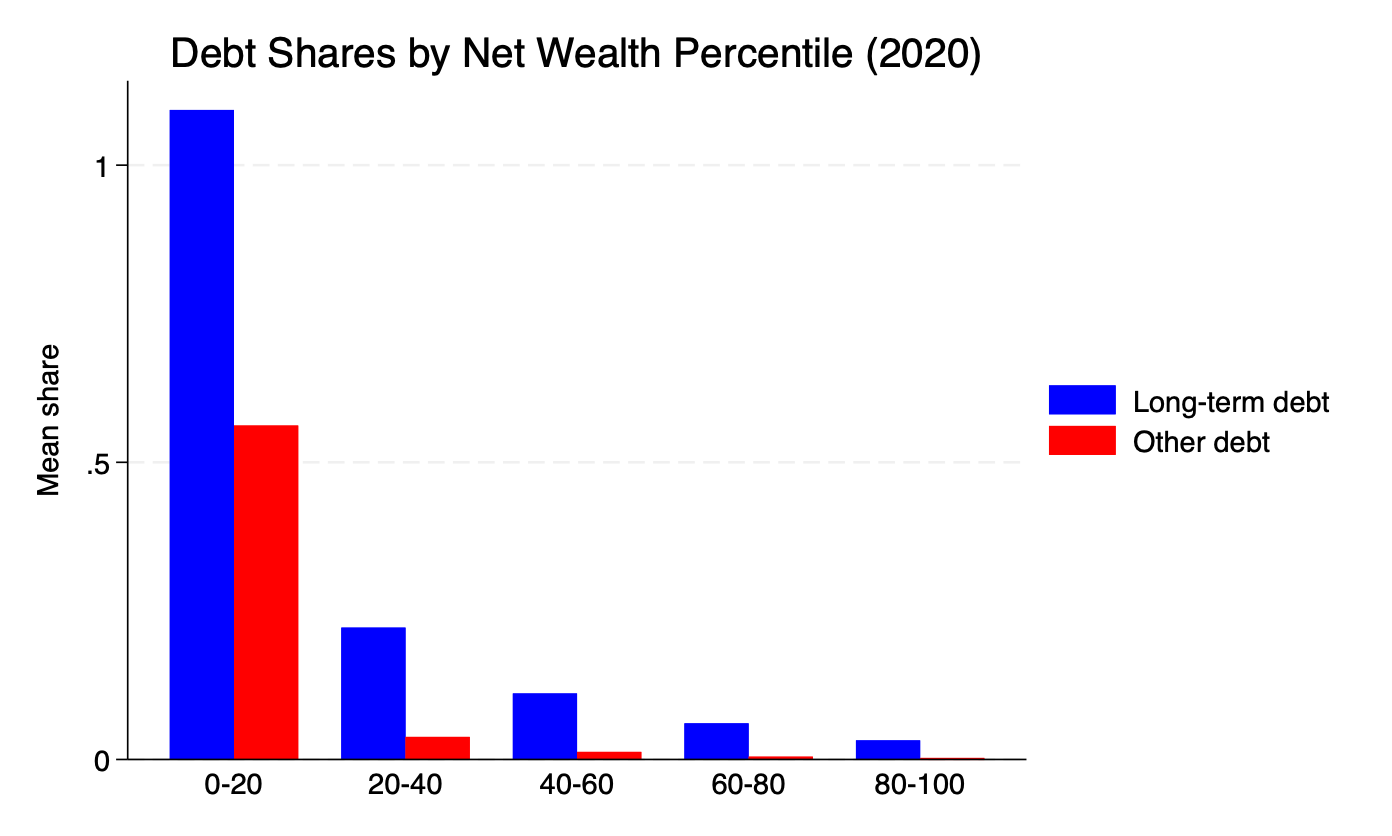
\includegraphics[width=0.8\textwidth]{../../Code/Descriptive/Figures/debt_shares_by_net_pct_2020.png}
\caption{Debt shares by net wealth percentile (2020)}
\end{figure}
\FloatBarrier

\par I summarize pooled participation and share statistics in Table~\ref{tab:summary_portfolios}.

\inputtable{../../Code/Regressions/Other/summary_portfolios.tex}
\label{tab:summary_portfolios}
\FloatBarrier

\par I also report pooled composition by wealth fractiles for the core distribution and for net wealth.

\inputtable{../../Code/Regressions/Other/asset_shares_by_wealth_frac.tex}
\label{tab:portfolio_comp_core_fractiles_pooled}
\FloatBarrier

\inputtable{../../Code/Regressions/Other/port_shares_by_wealth_frac.tex}
\label{tab:portfolio_comp_standard_fractiles_pooled}
\FloatBarrier

\subsection{Returns}

\par I follow recent literature using Norwegian administrative tax data at the population level and and using PSID in terms of the components used to construct a measure of returns. However, I take seriously the structure of the dataset I am working with(the HRS RAND longitudinal file) in defining the portfolio/asset class for which the returns are being accrued to. As mentioned before, core assets is the most narrowly defined asset class here because interest income and dividends does not disaggregate into the asset classes: stocks, bonds, private business, IRA/Keogh.

 The following formula from \cite{Daminato2024} serves as motivation for the return measures defined using the HRS data: $$ r_t = \frac{y^c_t + cg_t -F_t -y^d_t}{A_{t-1} + .5F_t}   $$ where $y^c_t$ interest income and dividends, capital gains $cg_t$ measured as the difference between reported stock across waves, $F_t$ net investment flows, $y^d_t$ payments on debt (in the RAND longitudinal file, the variables were mentioned are all in net terms so this variable was $0$), and $A_{t-1}$ total net wealth at beginning of previous period.
%%%%%%%%%%

 \subsubsection{Narrow asset classes}
 
\par Recall that we only see interest income and dividends for core assets and retirement assets. Since this is an important component of the returns calculation, we construct the narrowest return measure on core assets. To do so, I keep track of all asset classes captured in the capital gains variable\footnote{Those asset classes are: other real estate, business/farm, stocks/mutual funds, bonds, checking/savings, and CDs/t-bills.} and aggregate the capital gains and net investment flows for this group of assets.

\par Returns to core assets are given by

$$ r^{core}_{i,t} = \frac{y^{core}_{i,t} + cg^{core}_{i,t} - F^{core}_{i,t}}{A^{core}_{i,t-1} + .5F^{core}_{i,t}}   $$

where $y^{core}_{i,t}$ is the interest income and dividents on the core assets, $cg^{core}_{i,t}$ are the capital gains on the core assets\footnote{where the capital gains for each asset class is $V_{i,t} - V_{i,t-1}$, where $V_{i,t}$ is the value of the asset (business or stock or real estate) for the i-th respondent in the t-th wave of the survey.}, $F^{core}_{i,t}$ are the net investment flows on core assets, and importantly, $A^{core}_{i,t-1}$ is the total value of the core assets in the previous period.

\par The rest of the return measures are defined similarly. In the HRS data, we can see income on retirement assets as well. This allows us to define a return measure for retirement assets:

$$ r^{ret}_{i,t} = \frac{y^{ret}_{i,t} + cg^{ret}_{i,t} - F^{ret}_{i,t}}{A^{ret}_{i,t-1} + .5F^{ret}_{i,t}}   $$

where $y^{ret}_{i,t}$ is the interest income and dividents on the retirement assets, $cg^{ret}_{i,t}$ are the capital gains on the retirement assets, $F^{ret}_{i,t}$ are the net investment flows on retirement assets, and $A^{ret}_{i,t-1}$ is the total value of the retirement assets in the previous period.

\par Based on the modules offered in a given wave of the survey, assume that there are no interest income or dividends to either primary and secondary residential assets, so that the interest income and dividends accrued to residential assets is 0 in a given period $(y^{res}_{i,t}=0)$. With this in mind, returns to residential assets are defined as:

$$ r^{res}_{i,t} = \frac{cg^{res}_{i,t} - F^{res}_{i,t}}{A^{res}_{i,t-1} + .5F^{res}_{i,t}}   $$

where  $cg^{res}_{i,t}$ are the capital gains on the residential assets, $F^{res}_{i,t}$ are the net investment flows on residential assets (including improvement costs), and $A^{res}_{i,t-1}$ is the total value of the residential assets in the previous period.

\subsubsection{Broad asset classes}

\par After defining returns for narrow asset classes (i.e. returns to a single asset), I also define return measure for portfolios (returns on multiple assets). The first is for returns to both core and retirement assets: 

$$ r^{coret}_{i,t} = \frac{y^{coret}_{i,t} + cg^{coret}_{i,t} - F^{coret}_{i,t}}{A^{coret}_{i,t-1} + .5F^{coret}_{i,t}}   $$

where $y^{coret}_{i,t}$ is the interest income and dividends on core and retirement assets, $cg^{coret}_{i,t}$ are the capital gains on core and retirement assets, $F^{coret}_{i,t}$ are the net investment flows on core and retirement assets, and $A^{coret}_{i,t-1}$ is the total value of core and retirement assets in the previous period.

\par Returns to net wealth is given by

$$ r^{net}_{i,t} = \frac{y^{net}_{i,t} + cg^{net}_{i,t} - F^{net}_{i,t}}{A^{net}_{i,t-1} + .5F^{net}_{i,t}}   $$

where $y^{net}_{i,t}$ is the interest income and dividends on core and retirement assets, $cg^{net}_{i,t}$ are the capital gains on all available asset classes in the survey, $F^{net}_{i,t}$ are the net investment flows on assets for which it is relevant in the survey (stocks, bonds, business, IRA, residences, and real estate), and $A^{net}_{i,t-1}$ is the total value of the available assets minus liabilities in the previous period\footnote{Mortgages on secondary residences are left out of the list of liabilities since it was an optional question in some waves of the survey.}.

\par I present the means for the return measures in the following figure ~\ref{fig:returns_mean_by_year_panels}. I group them by the returns at the asset level (core, retirement, residential) and at the portfolio level (core, core and retirement, net wealth). %%%%describe%%%%%%

\begin{figure}[H]
\centering
\begin{minipage}[t]{0.48\textwidth}
\centering
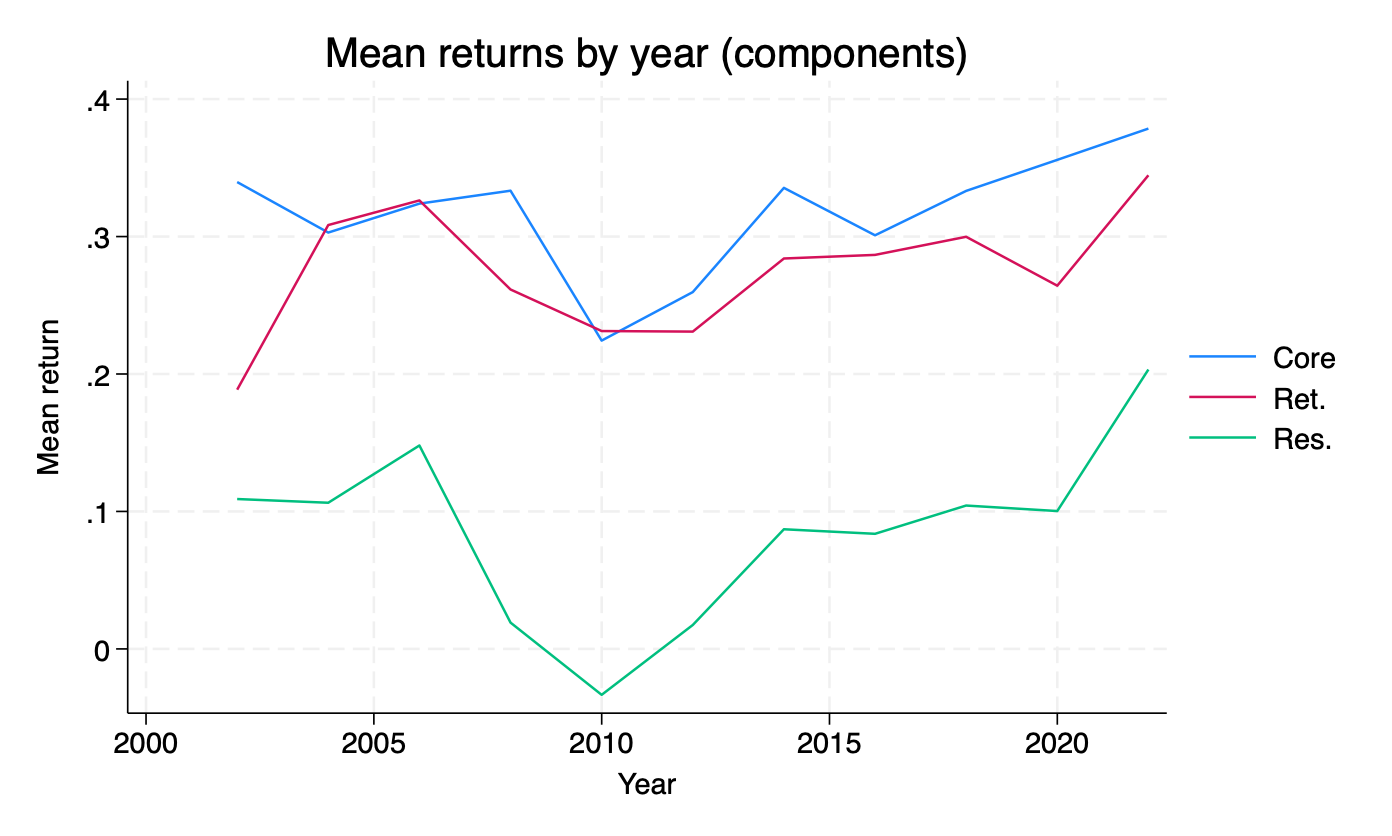
\includegraphics[width=\textwidth]{../../Code/Descriptive/Figures/returns_mean_by_year_components.png}
\end{minipage}\hfill
\begin{minipage}[t]{0.48\textwidth}
\centering
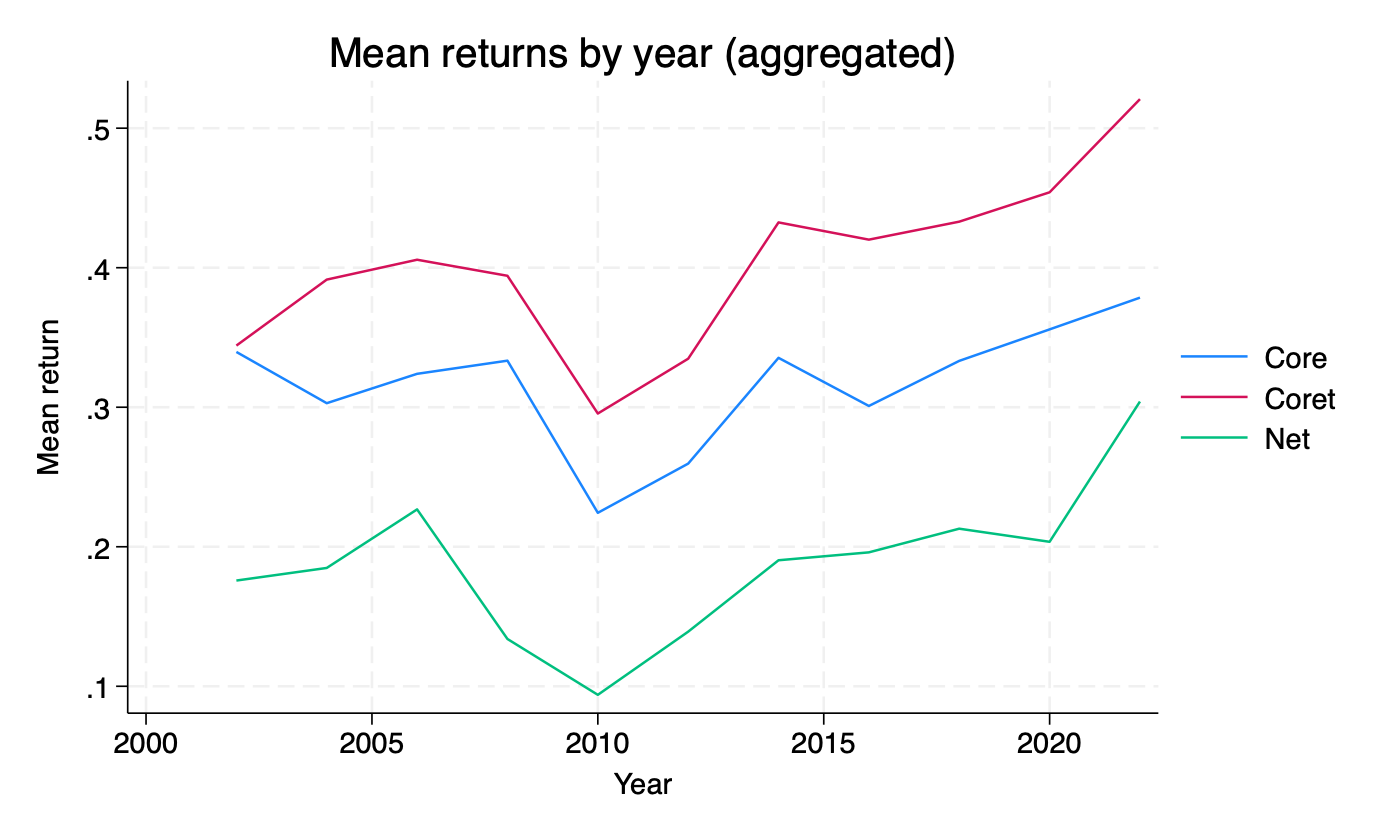
\includegraphics[width=\textwidth]{../../Code/Descriptive/Figures/returns_mean_by_year_agg.png}
\end{minipage}
\caption{Mean returns by year}
\label{fig:returns_mean_by_year_panels}
\end{figure}
\FloatBarrier

Figure ~\ref{fig:returns_histogram_agg_2022} shows the distribution of the return measures across respondents by a similar grouping. In general, this attempt is encouraging, as its shape (in particular, for returns to net wealth) closely resembles early estimates of the empirical distribution of individual realized returns in the Norwegian population data. 

\begin{figure}[H]
\centering
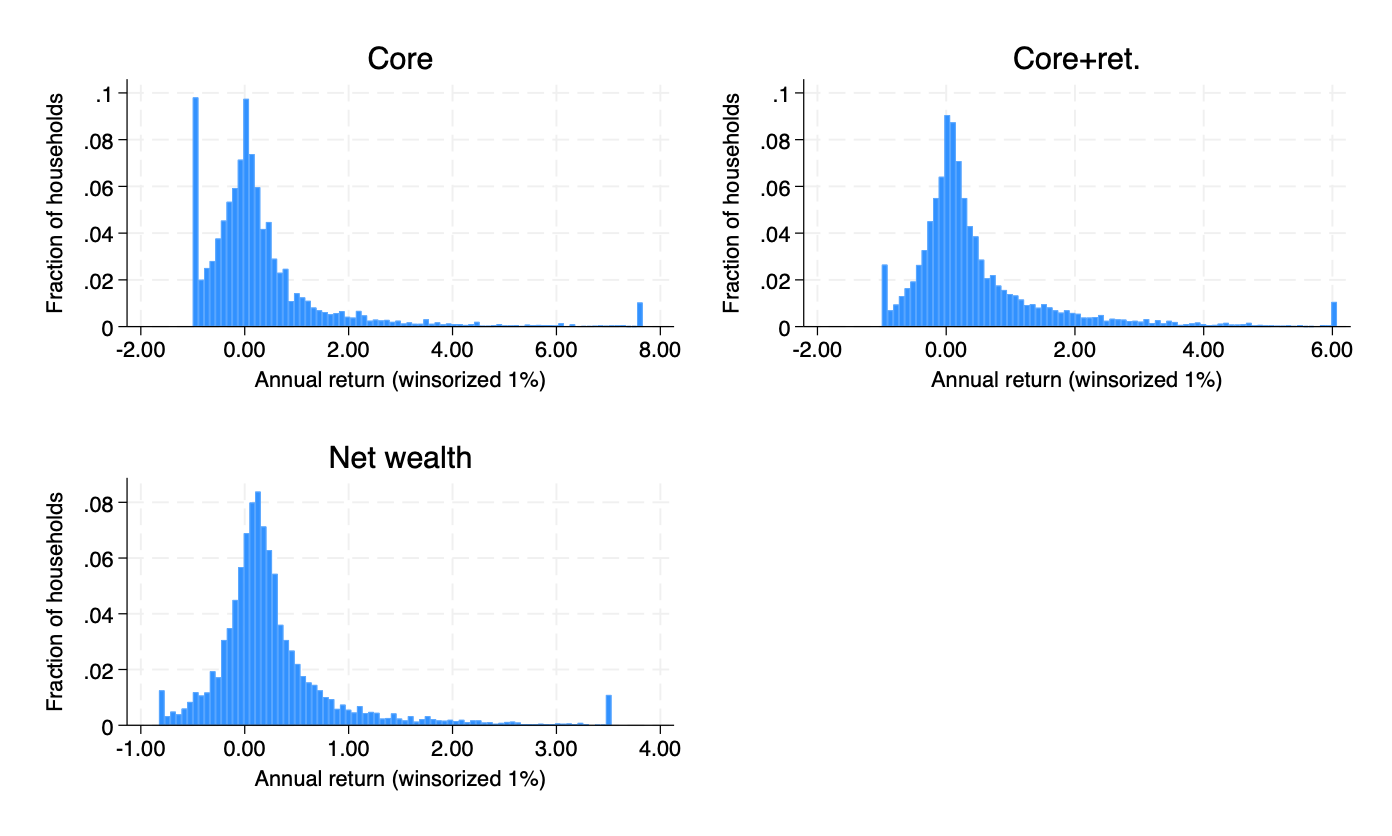
\includegraphics[width=0.8\textwidth]{../../Code/Descriptive/Figures/returns_histogram_agg_2022.png}
\caption{Returns histogram, aggregated (2022)}
\label{fig:returns_histogram_agg_2022}
\end{figure}
\FloatBarrier

\par %%%describe%%%

\par %%%describe, for components below%%%

\begin{figure}[H]
\centering
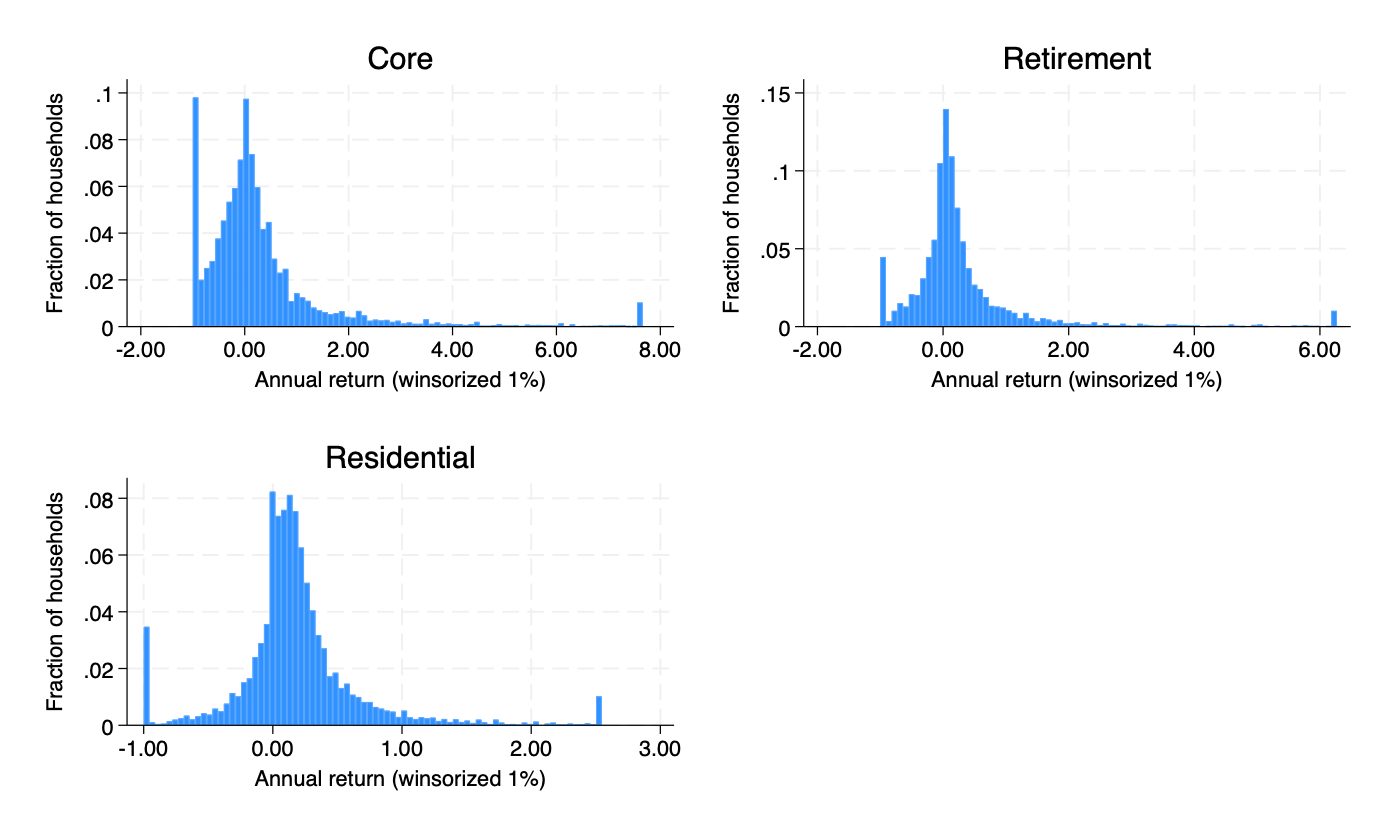
\includegraphics[width=0.8\textwidth]{../../Code/Descriptive/Figures/returns_histogram_components_2022.png}
\caption{Returns histogram, components (2022)}
\end{figure}
\FloatBarrier

\par %%short paragraph about outliers - come back to this%%

\par %%describe table about the dist of returns summary %%%%

\inputtable{../../Code/Regressions/Other/returns_portfolio_moments_pooled.tex}
\label{tab:returns_portfolio_moments_pooled}
\FloatBarrier

\subsection{Income and wealth}

\par Income and wealth are understood to be positively correlated. To see this play out in the HRS data, I first look at mean labor income by wealth percentile. In ths figure, it is clear that a positive relationship seems to hold. 

\begin{figure}[H]
\centering
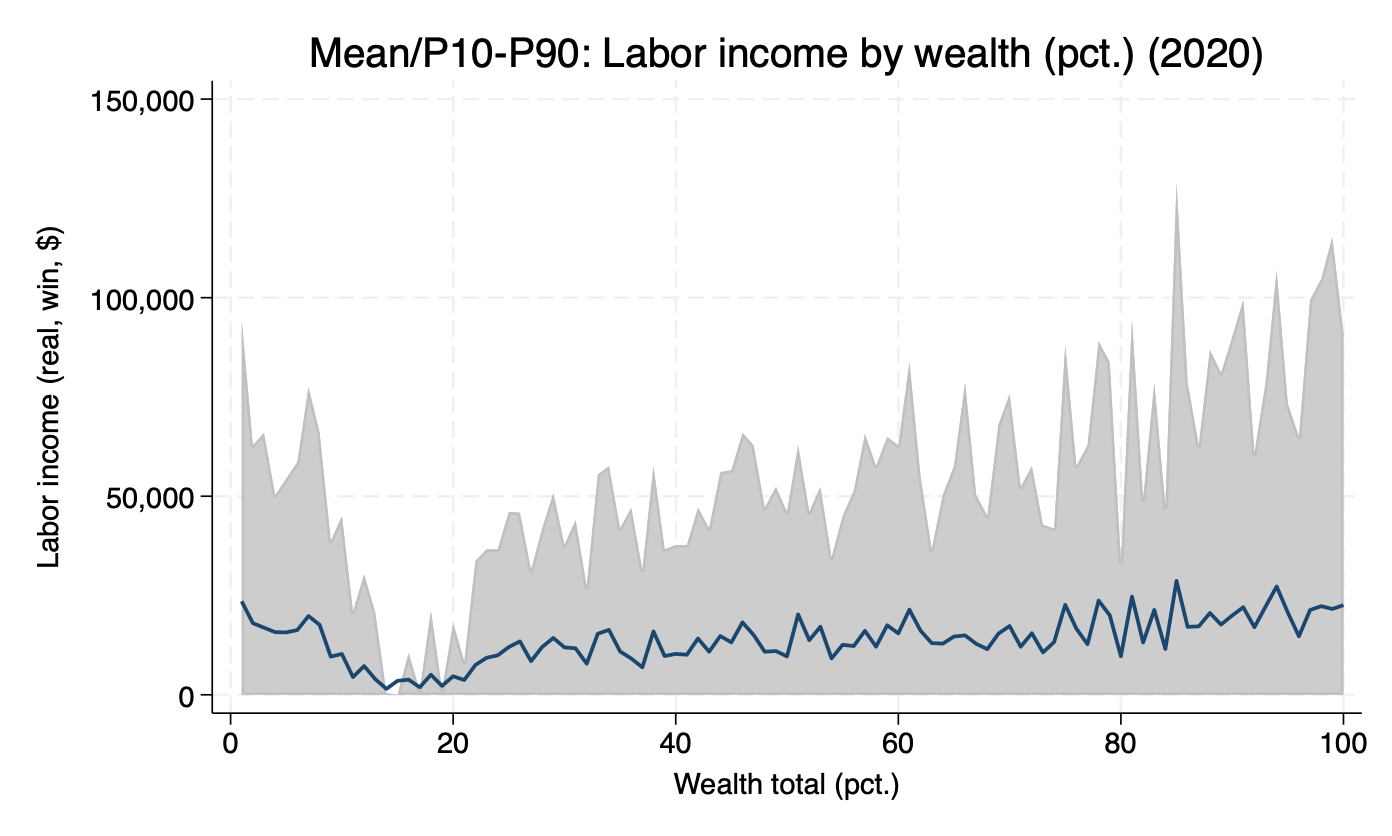
\includegraphics[width=0.8\textwidth]{../../Code/Descriptive/Figures/labor_income_real_win_p10p90_by_wealthpct_2020.png}
\caption{Labor income mean/P10-P90 by wealth percentile (2020)}
\end{figure}
\FloatBarrier 

The literature on income and wealth also documents significantly more inequality in the the upper tails of the wealth distribution than in the income distribution. The observations towards to top and bottom of the wealth distribution in the following figure seem to suggest a non-linear relationship between the variables. This pattern can be better seen in the figure ~\ref{total_income_real_win_iqr_by_wealthpct_2020}.

\begin{figure}[H]
\centering
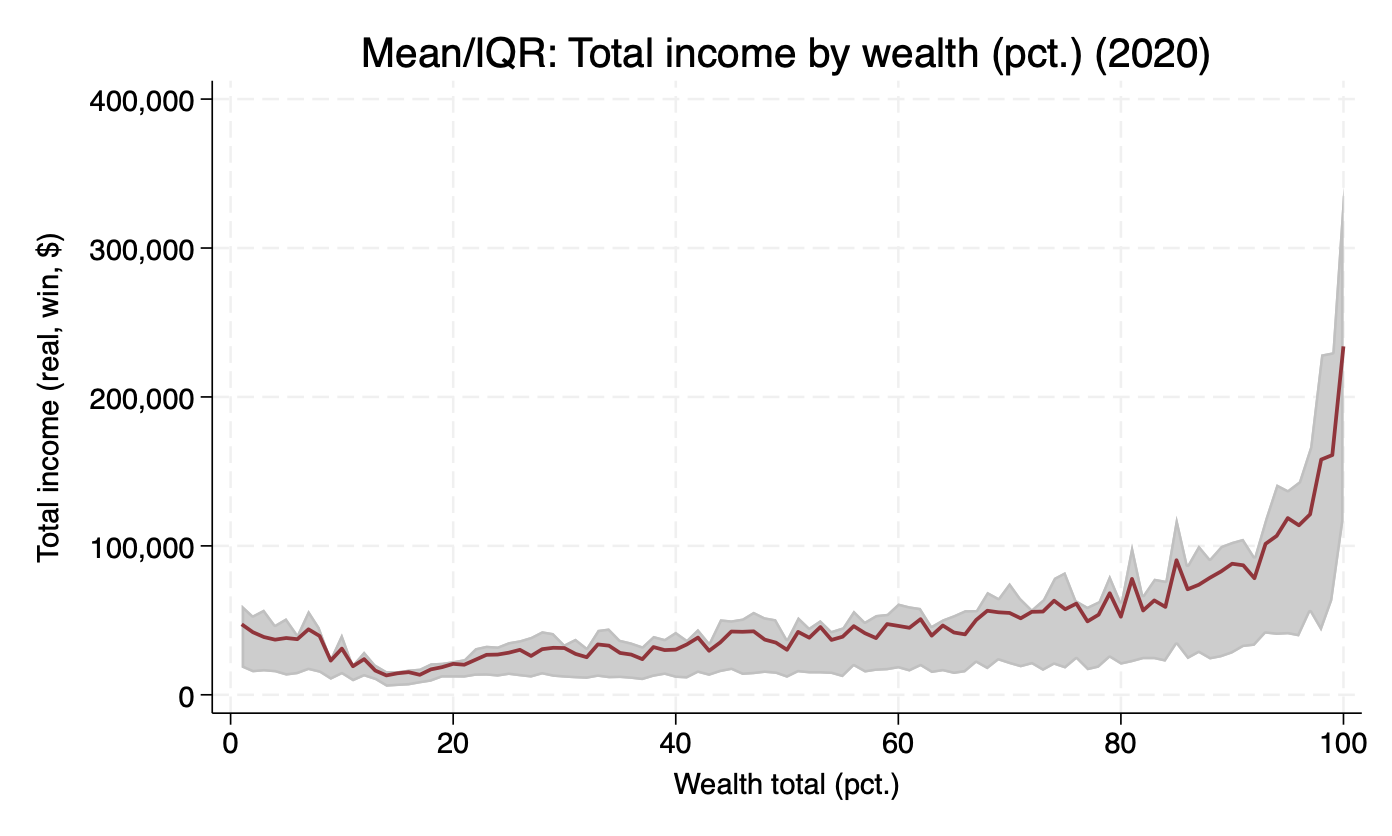
\includegraphics[width=0.8\textwidth]{../../Code/Descriptive/Figures/total_income_real_win_iqr_by_wealthpct_2020.png}
\caption{Total income mean/IQR by wealth percentile (2020)}
\label{total_income_real_win_iqr_by_wealthpct_2020}
\end{figure}
\FloatBarrier


\subsection{Returns and wealth by portfolio}

\par A positive relationship between wealth and returns has also been documented, referred to as \textit{scale dependence}. In the next three figures, I show that there does seem to be a positive statistical relationship between the return measure (core, retirement, residential) and wealth. 

\begin{figure}[H]
\centering
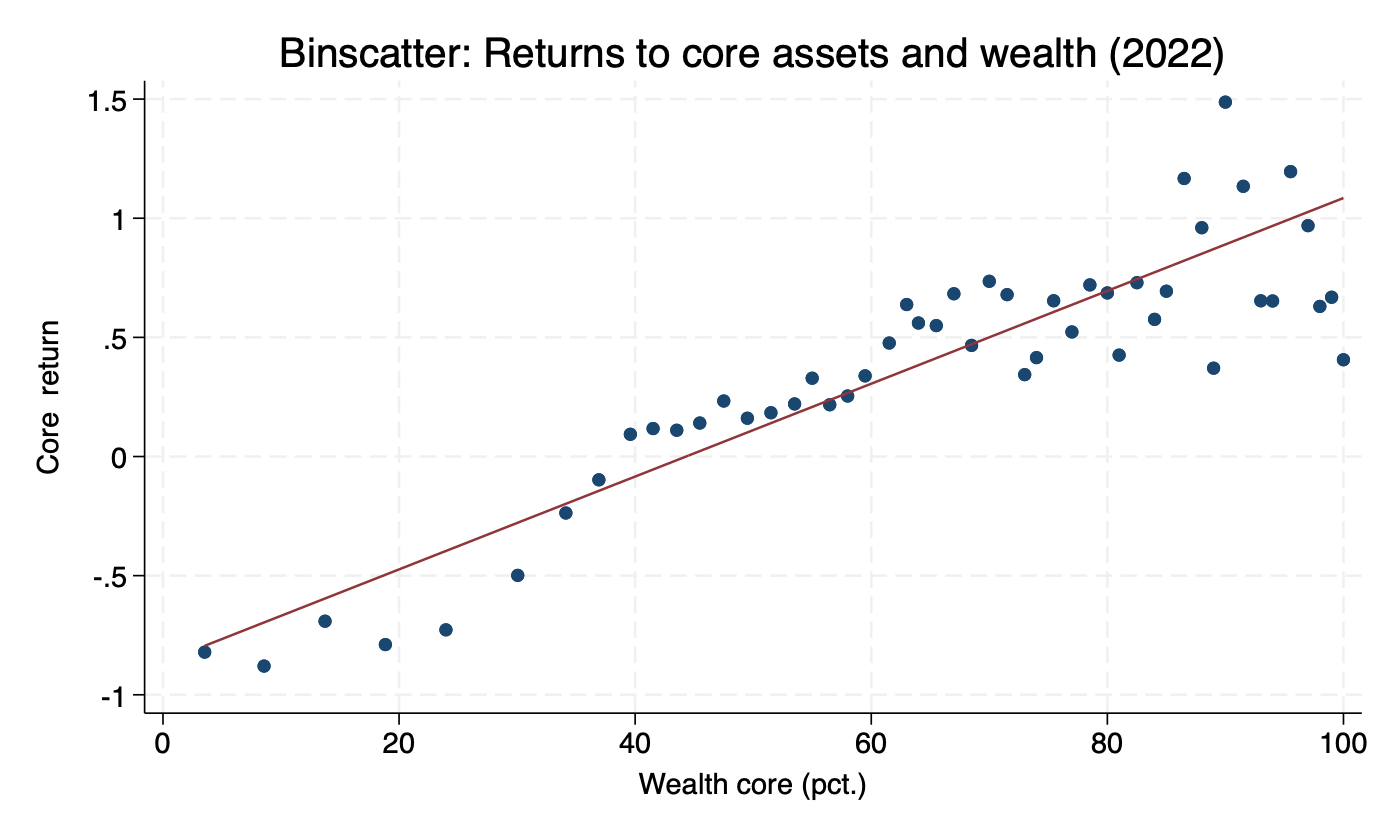
\includegraphics[width=0.8\textwidth]{../../Code/Descriptive/Figures/core_return_binscatter_2022.png}
\caption{Core return binscatter (2022)}
\end{figure}
\FloatBarrier

\begin{figure}[H]
\centering
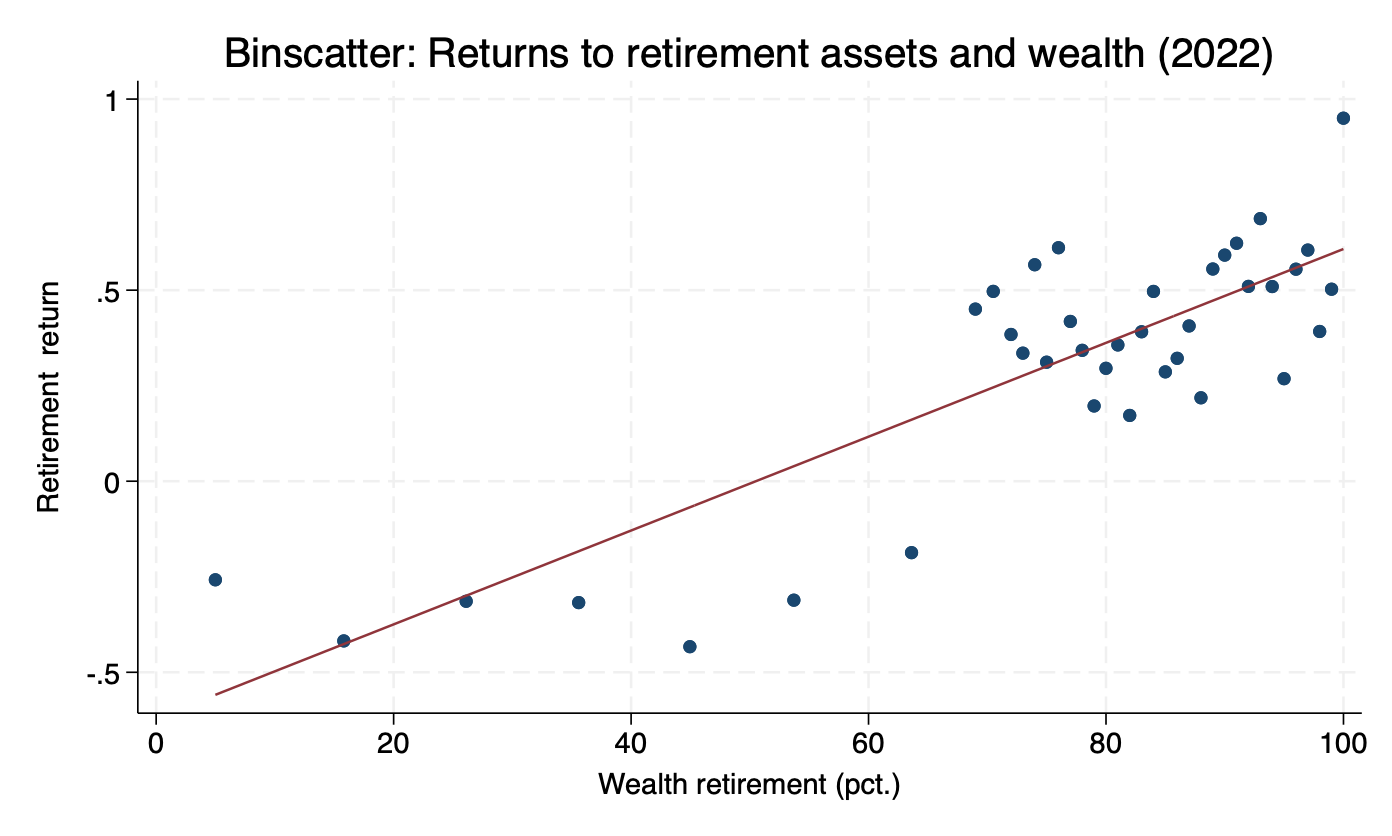
\includegraphics[width=0.8\textwidth]{../../Code/Descriptive/Figures/ret_return_binscatter_2022.png}
\caption{Retirement return binscatter (2022)}
\end{figure}
\FloatBarrier

\begin{figure}[H]
\centering
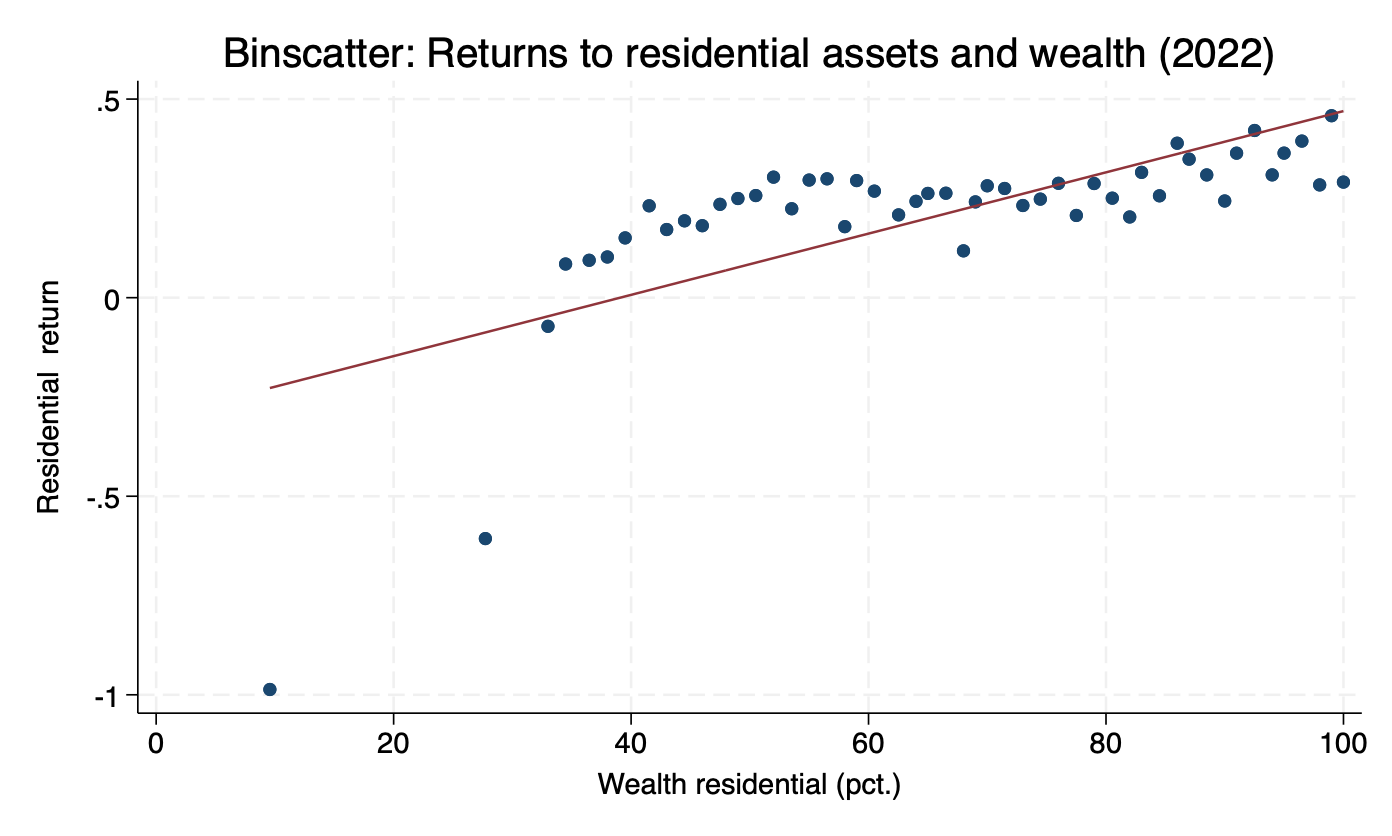
\includegraphics[width=0.8\textwidth]{../../Code/Descriptive/Figures/res_return_binscatter_2022.png}
\caption{Residential return binscatter (2022)}
\end{figure}
\FloatBarrier

\par I also show the positive statistical relationship between returns and wealth at the portfolio level, when comprised of core assets and retirement assets. 

\begin{figure}[H]
\centering
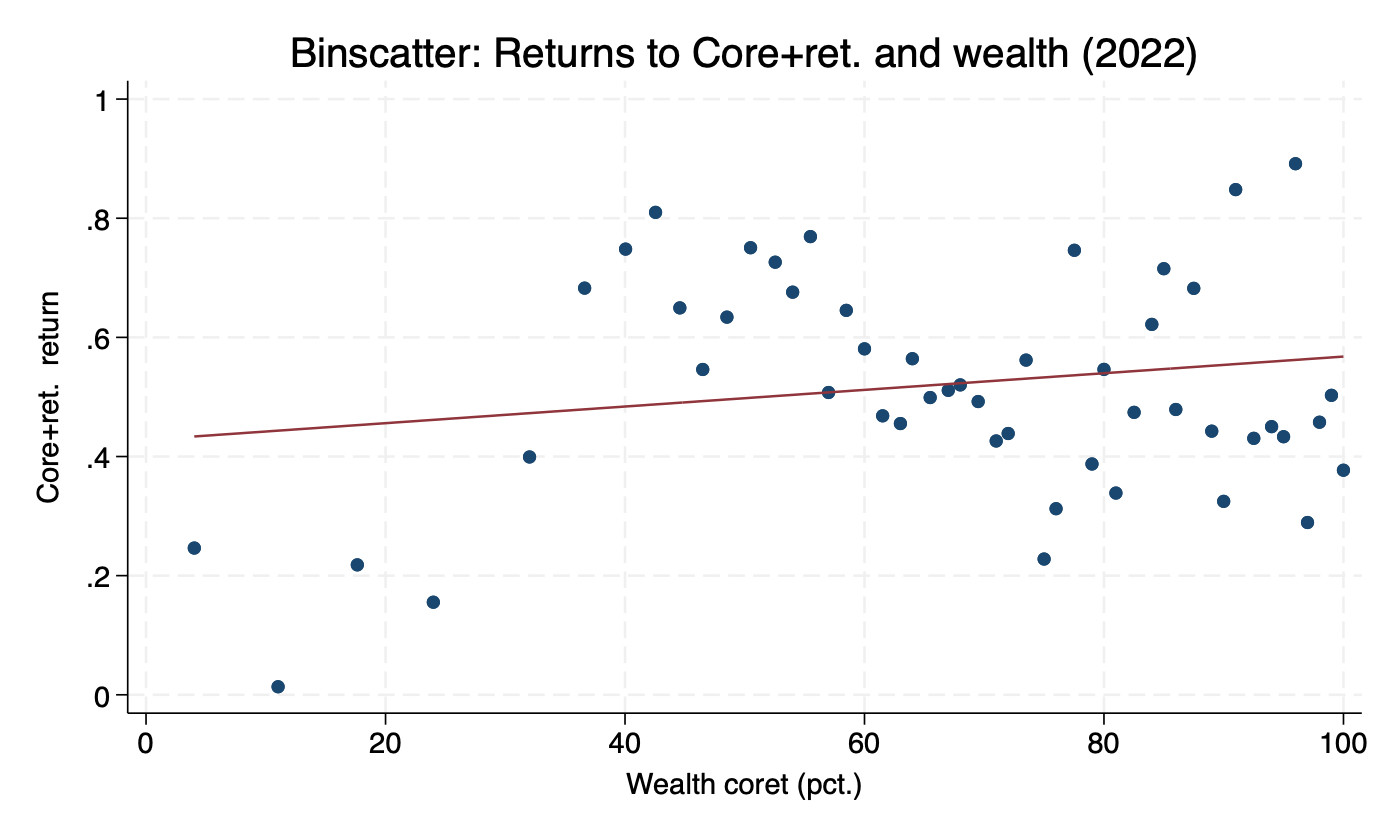
\includegraphics[width=0.8\textwidth]{../../Code/Descriptive/Figures/coreira_return_binscatter_2022.png}
\caption{Core+IRA return binscatter (2022)}
\end{figure}
\FloatBarrier

\par Interestingly, the relationship between wealth and returns to total net wealth does not appear positive. In fact, they correlation is slightly downward-sloping.

\begin{figure}[H]
\centering
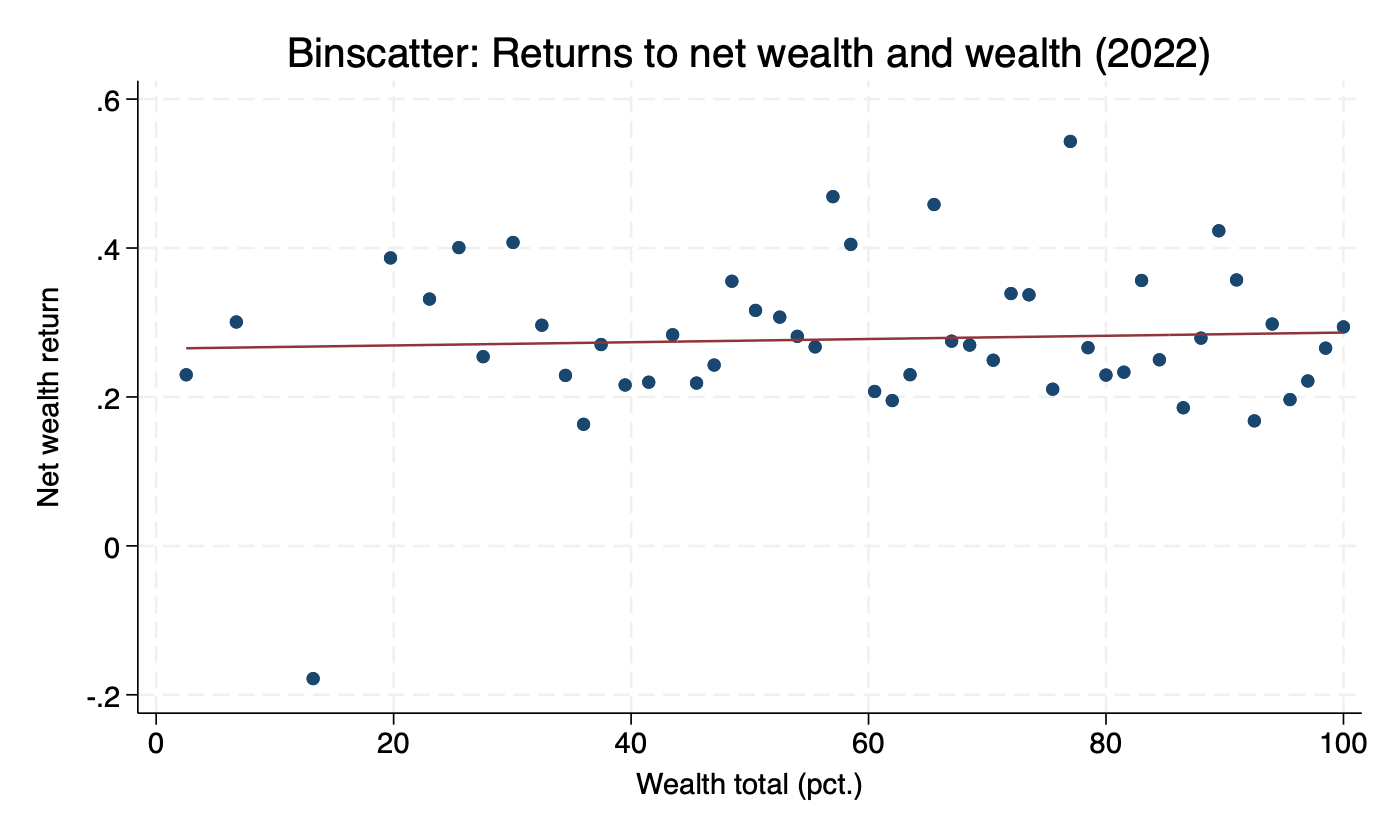
\includegraphics[width=0.8\textwidth]{../../Code/Descriptive/Figures/netwealth_return_binscatter_2022.png}
\caption{Net wealth return binscatter (2022)}
\end{figure}
\FloatBarrier

\subsection{Trust}

\par I turn my attention to the suite of trust questions in \say{Section V: Modules} section of the 2020 HRS data. There are a total of 8 questions, asking respondents to say on a scale of 1-10 \say{how much do you trust people in general?} and of their trust in other features of American life relating to healthcare, finance, and media. These questions were only asked for a single year. Although this is an issue, because the panel structure of the HRS allows me to estimate the persistent component of returns, which is an important object in this literature. That said, in the pooled setting, we can assume that trust, like education, is fixed over time.\footnote{Literature on trust talks about how history of being cheated or treated fairly form individuals' trust over time. If this is true and at some point, one learns enough an forms their trust level, then a sample with an overrepresentation of older household is a reasonable environment to assume constant trust levels.}

\par I summarize general trust by age, gender, race, and education in Table~\ref{tab:trust_general_demographics_panels}. %%summarize

\inputtable{../../Code/Descriptive/Tables/trust_general_demographics_panels.tex}
\label{tab:trust_general_demographics_panels}

\par I am interested in the relationship between trust and economic performance as the literature is, however in my setting the measure of economic performance is the return to assets. If a hump-shaped relationship is reasonable for income, it is even more plausible for returns: there is an inherent (and possibly explicit) level of trust between borrower and lender when forming credit contracts.

% \par That said, it is important to understand the nature of the trust measure in the HRS sample. I begin to do this by considering each trust measure conditional on race/ethnicity. There seems to be significant group variation in means.

% \begin{figure}[H]
% \centering
% 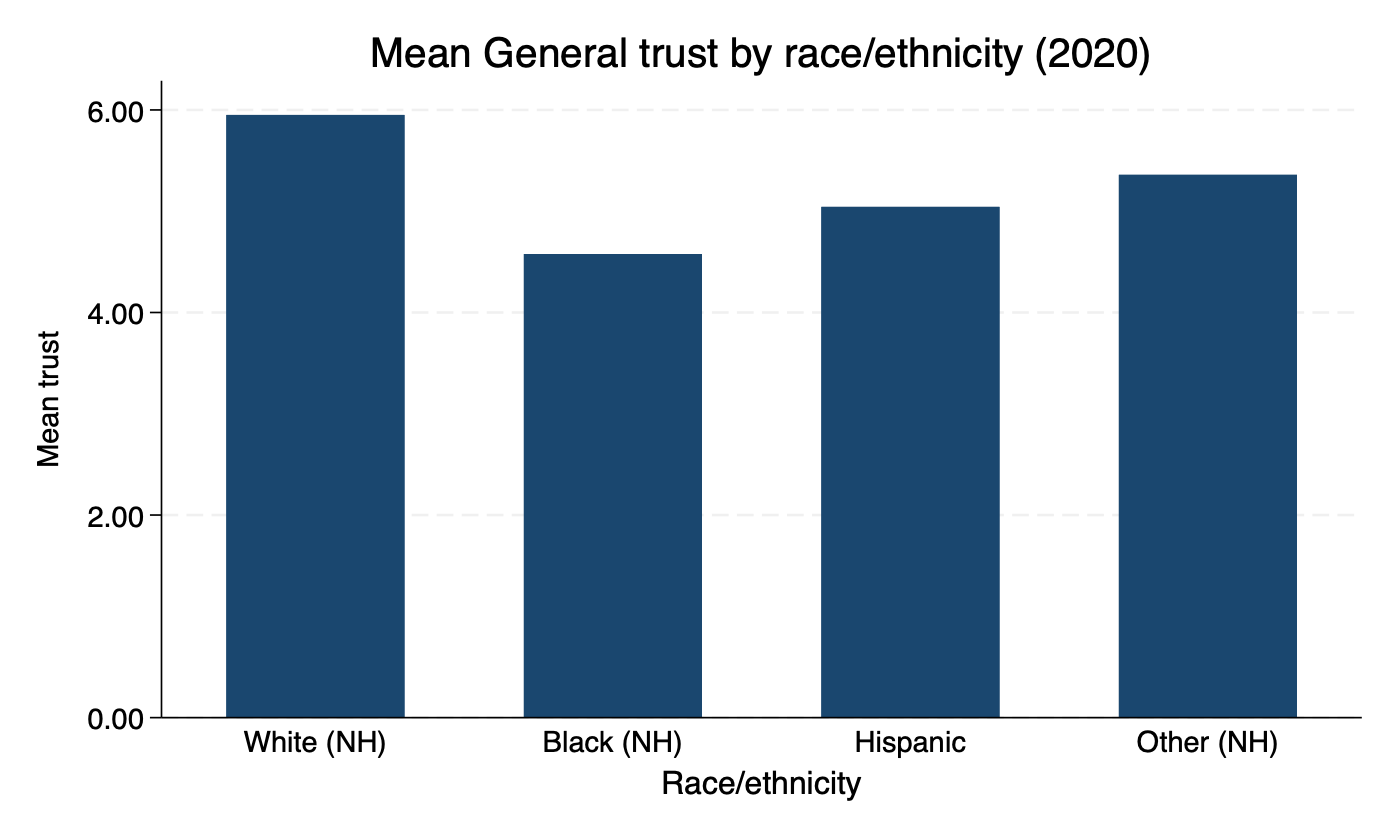
\includegraphics[width=0.8\textwidth]{../../Code/Descriptive/Figures/trust_mean_by_race_eth_others_2020.png}
% \caption{Mean general trust by race/ethnicity (2020)}
% \end{figure}
% \FloatBarrier

\subsubsection{Trust and income}

\par As discussed before, the literature on trust and economic performance suggests there's a \say{right amount of trust}. I want to see if this hump shaped relationship holds between the measures of trust and income in the HRS. After deflating and, more importantly, winsorizing labor income at the top and bottom 1\%, the relationship seems to be hump shaped.

\par Income in the HRS is highly right-skewed and features a large mass at zero labor income (reflecting retirement and non-participation). In applied work, a common baseline is to use $\log(\text{income})$ because it reduces the influence of extreme values and yields coefficients interpretable as semi-elasticities. However, $\log(\cdot)$ is undefined at zero (and problematic with negative values when they arise from measurement or netting conventions), so using $\log(\text{income})$ in the HRS mechanically drops a large fraction of observations and can substantially change the visual and econometric relationship.

\par In our data, the corresponding scatter of $\log(\text{income})$ versus trust changes markedly because so many observations have exactly zero labor income. Using $\log(1+\text{income})$ retains zeros but imposes an ad hoc curvature near zero and, in our case, does not restore the same qualitative picture.

\begin{figure}[H]
\centering
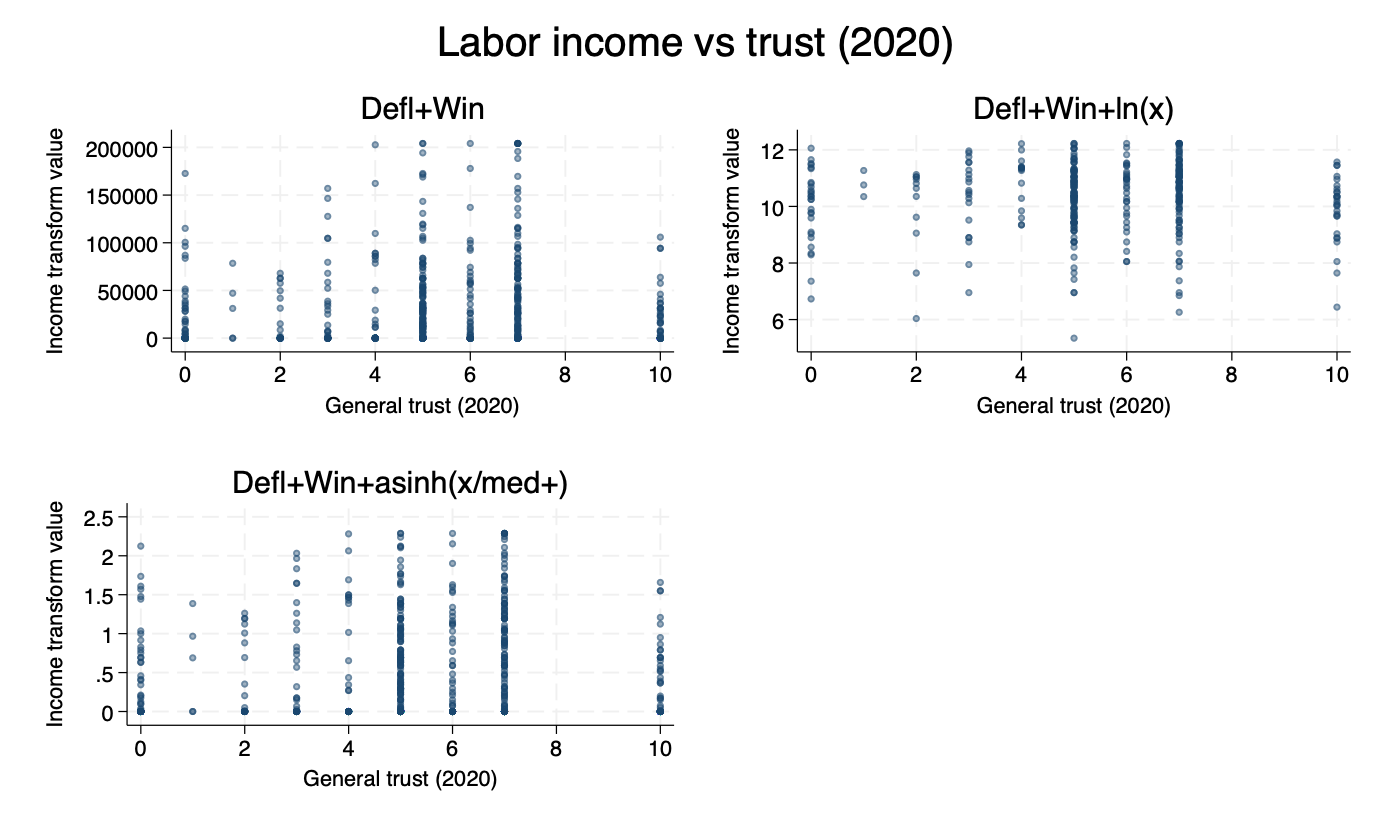
\includegraphics[width=0.8\textwidth]{../../Code/Descriptive/Figures/dw_lab_trust_2020.png}
\caption{Labor income measures vs.\ trust (2020)}
\end{figure}
\FloatBarrier 

\par Motivated by this issue, we follow a large applied econometrics literature that uses the inverse hyperbolic sine (IHS, or $\operatorname{asinh}$) transformation as a ``log-like'' mapping that is well-defined at zero and can accommodate negative values. The IHS transformation was advocated early on as an alternative to the log for heavy-tailed outcomes with extreme values and potential zeros/negatives (Burbidge, Magee, and Robb, \emph{``Alternative Transformations to Handle Extreme Values of the Dependent Variable''}; MacKinnon and Magee, \emph{``Transforming the Dependent Variable in Regression Models''}). More recently, Bellemare and Wichman (\emph{``Elasticities and the Inverse Hyperbolic Sine Transformation''}) provide practical guidance on interpretation, emphasizing that $\operatorname{asinh}(y)$ behaves similarly to $\log(y)$ for large $y$ (since $\operatorname{asinh}(y)\approx \log(2y)$ when $y$ is large) while remaining defined at $y=0$.

\par A related point is that the IHS can be sensitive to the units of measurement, which motivates a \emph{scaled} IHS of the form $\operatorname{asinh}(y/\kappa)$ (see discussions in A\"ihounton and Henningsen, \emph{``Units of Measurement and the Inverse Hyperbolic Sine Transformation''}; Norton, \emph{``The Inverse Hyperbolic Sine Transformation''}). In practice, $\kappa$ is chosen as a meaningful scale (e.g., the median positive income), which makes the transformation more comparable across samples and improves interpretability near zero. Empirically, applying the (scaled) IHS to our deflated and winsorized income restores a scatter with trust that is visually well-behaved while retaining the economically important mass at zero labor income. This can be seen for the measure of toal income as well in the following figure .


\begin{figure}[H]
\centering
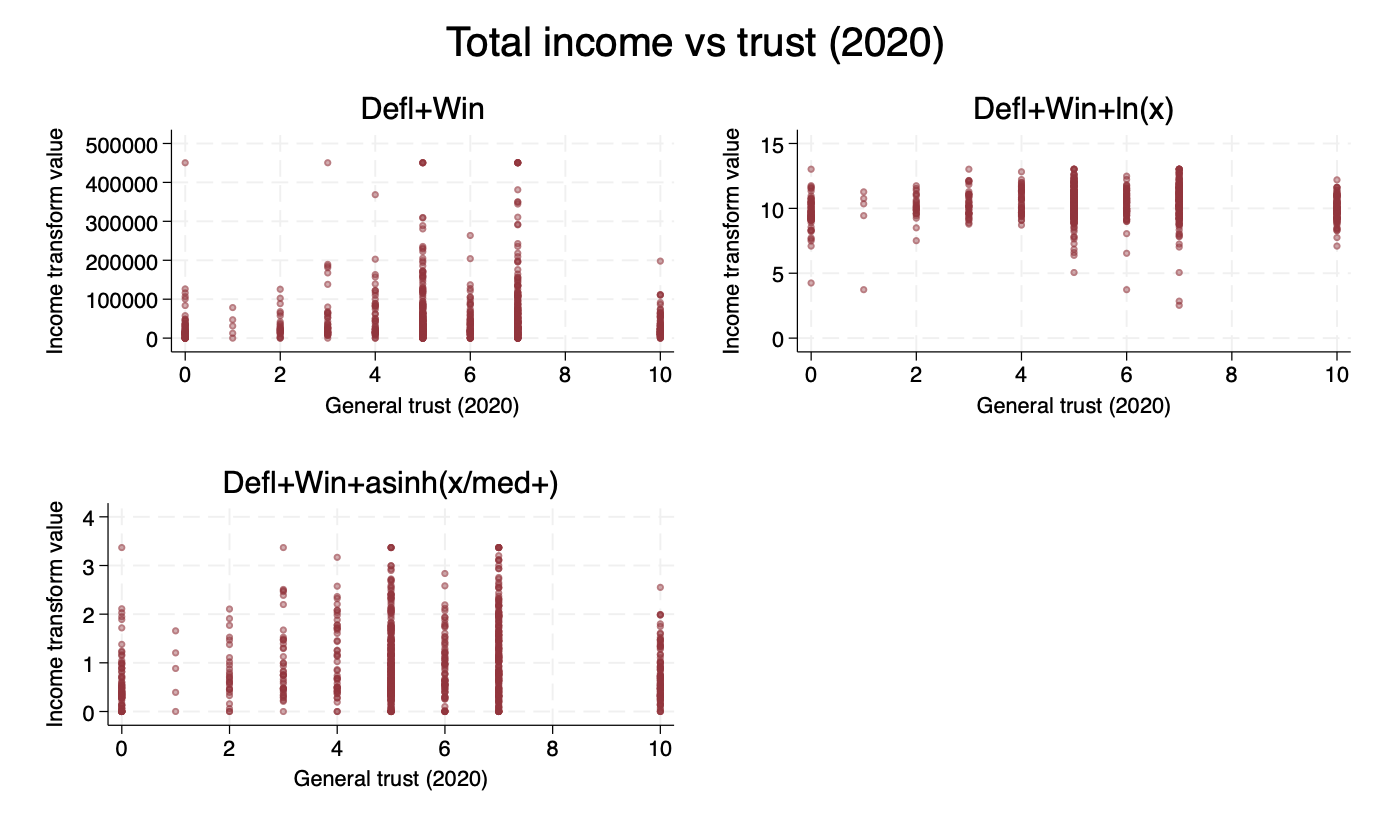
\includegraphics[width=0.8\textwidth]{../../Code/Descriptive/Figures/dw_tot_trust_2020.png}
\caption{Total income measures vs.\ trust (2020)}
\end{figure}
\FloatBarrier

%%%%%%

\subsubsection{Trust and returns}

\par The scatterplots for trust and the measures of returns suggest stronger evidence for this hump shaped relationship. Especially for the smaller portfolio compositions (core, core and retirement), return values are highest in the middle and lower at the lowest and highest trust values.

\begin{figure}[H]
\centering
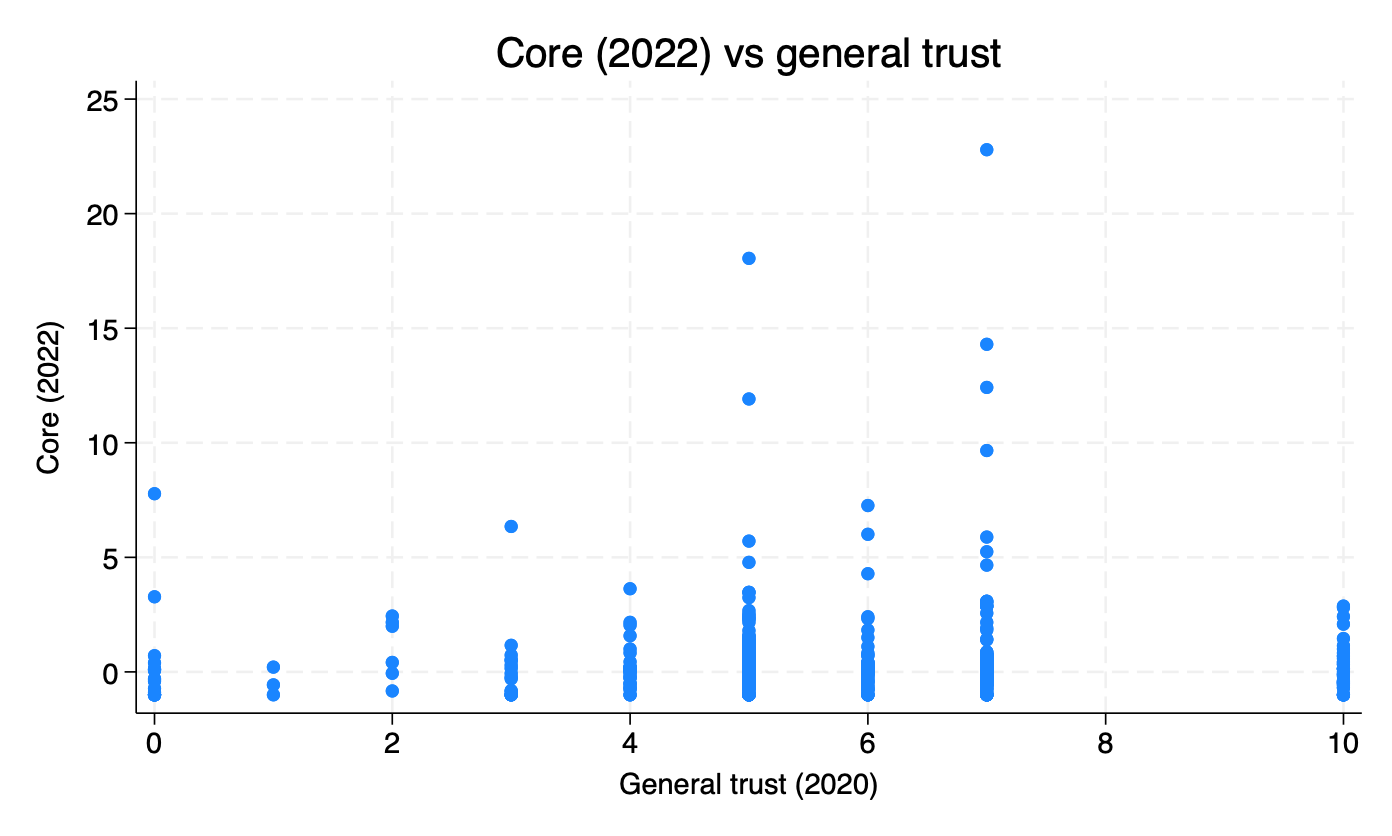
\includegraphics[width=0.8\textwidth]{../../Code/Descriptive/Figures/r1_annual_2022_vs_trust_2022.png}
\caption{Returns to core assets vs.\ trust (2022)}
\end{figure}
\FloatBarrier

\begin{figure}[H]
\centering
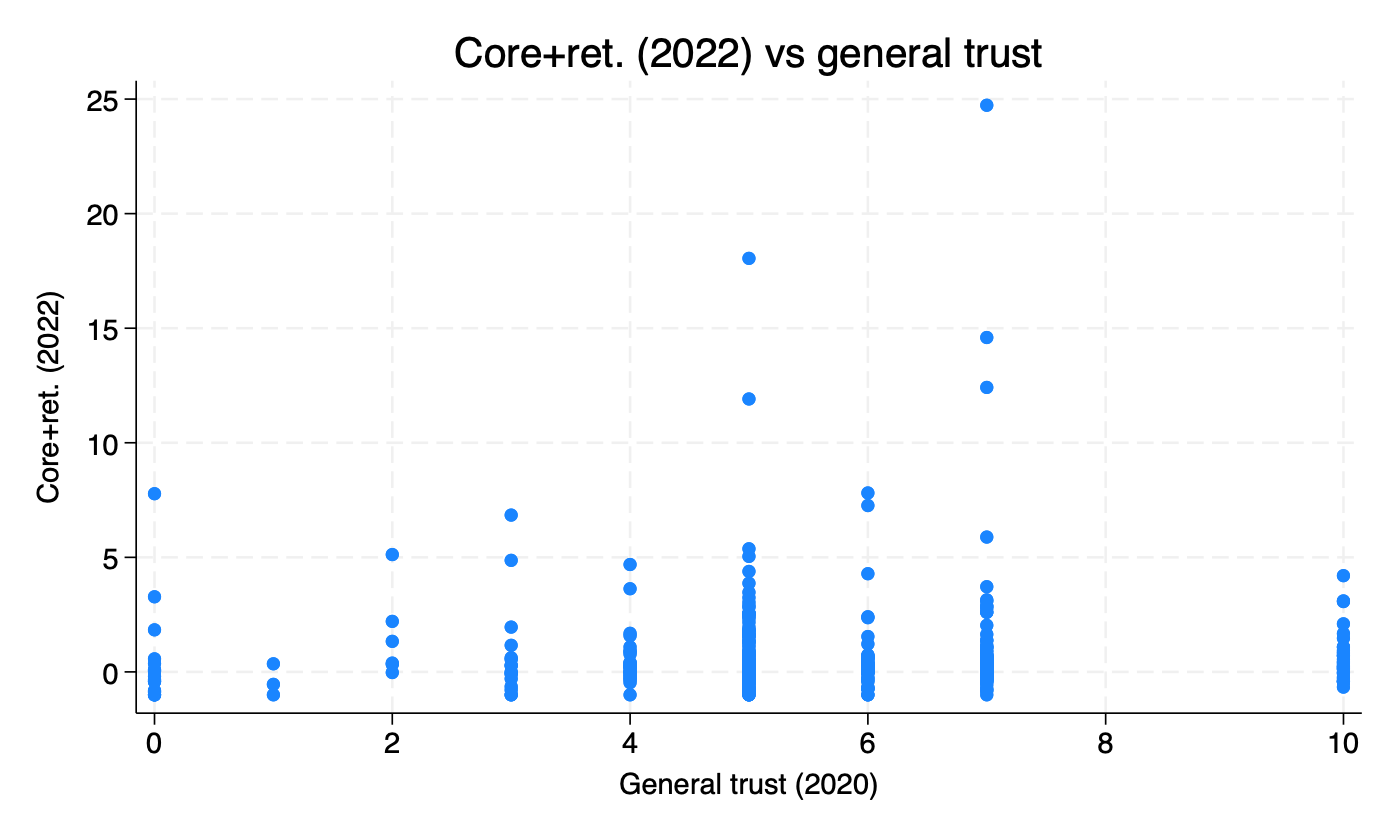
\includegraphics[width=0.8\textwidth]{../../Code/Descriptive/Figures/r4_annual_2022_vs_trust_2022.png}
\caption{Returns to core and retirement assets vs.\ trust (2022)}
\end{figure}
\FloatBarrier

\begin{figure}[H]
\centering
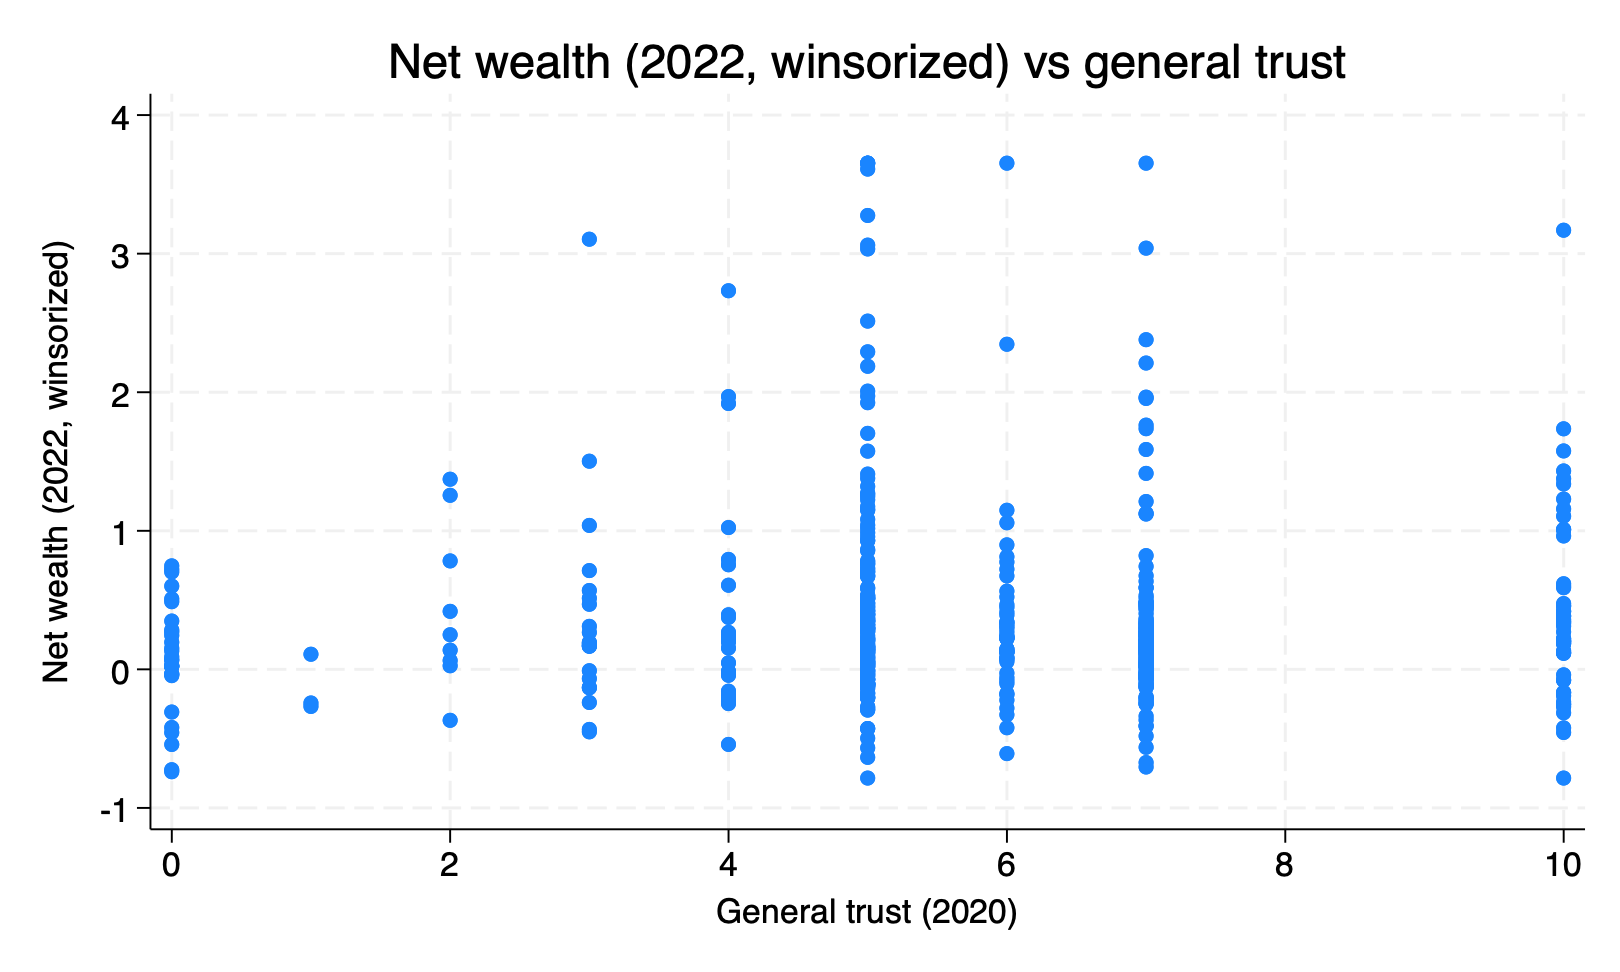
\includegraphics[width=0.8\textwidth]{../../Code/Descriptive/Figures/r5_annual_2022_win_vs_trust_2022.png}
\caption{Returns to net wealth vs.\ trust (2022)}
\end{figure}
\FloatBarrier

\subsection{Demographics}

\par As the HRS oversample older households, I take a quick look at demographic variables that will be important for the statistical analysis later. 

\begin{table}[H]
\centering
\textit{Panel A: Demographics (general)}\\[0.3em]
\input{../../Code/Descriptive/Tables/demographics_general_tabular.tex}

\vspace{0.8em}
\textit{Panel B: Demographics (other controls)}\\[0.3em]
\input{../../Code/Descriptive/Tables/demographics_other_tabular.tex}
\caption{Demographic summary statistics}
\label{tab:demographics_panels}
\end{table}
\par The literature on trust already documents a signficant statistical relationship between trust and mental health. For that reason, I use the HRS RAND measure for a mental health index and show a clearly negative, linear relationship with trust. 

\begin{figure}[H]
\centering
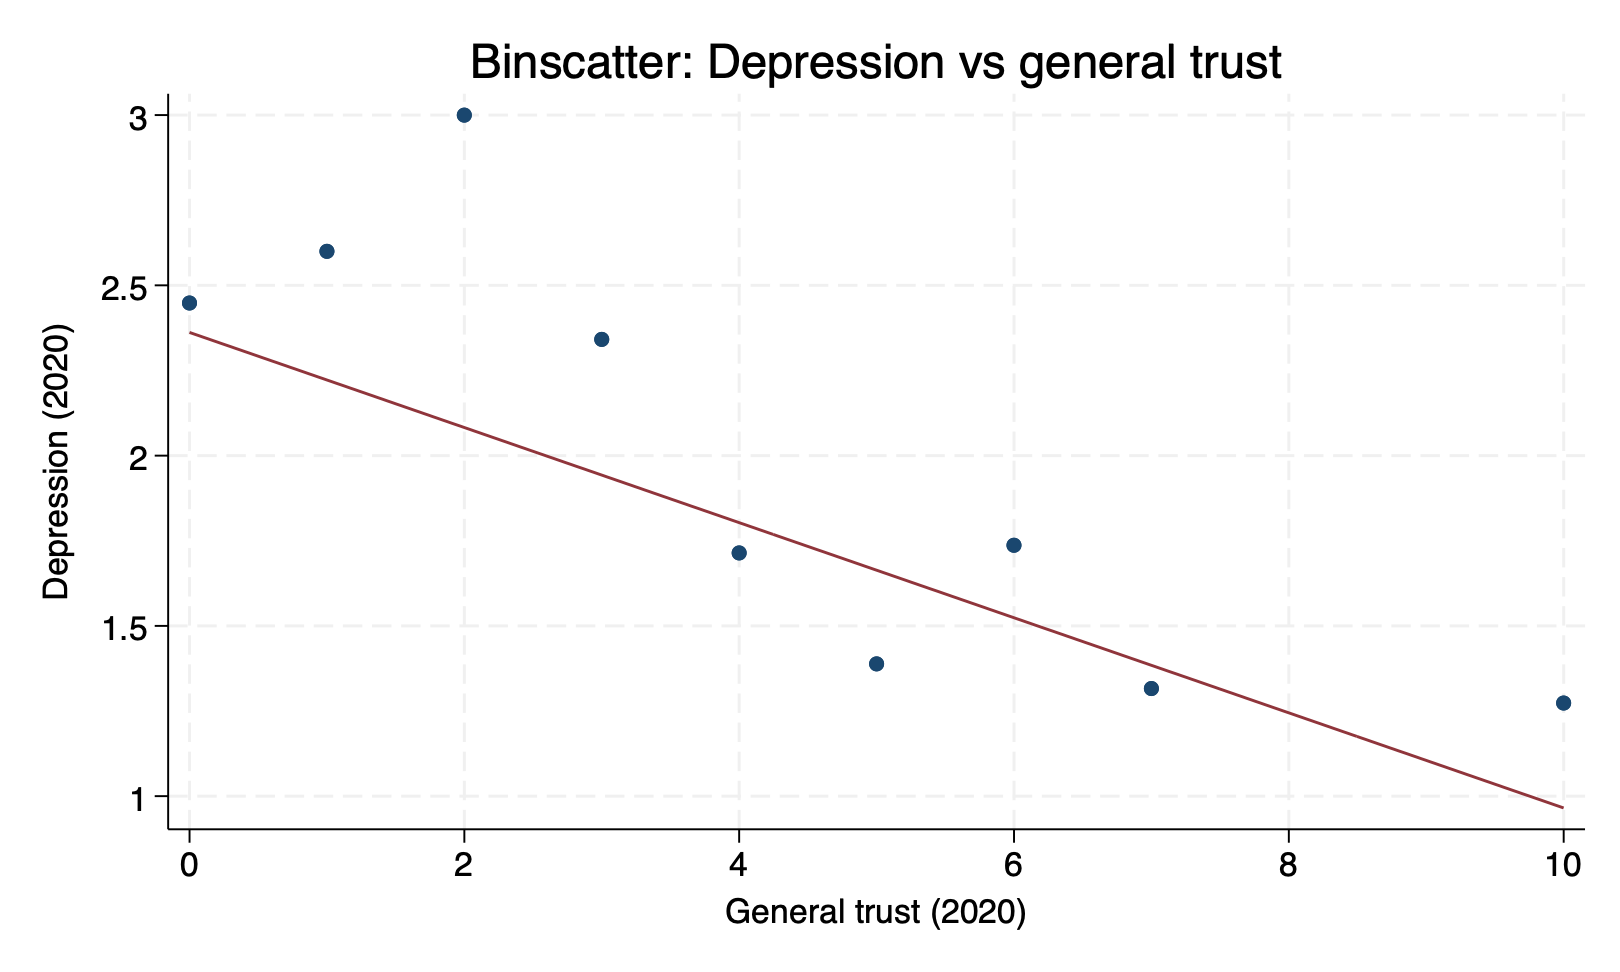
\includegraphics[width=0.8\textwidth]{../../Code/Descriptive/Figures/depression_vs_trust_binscatter.png}
\caption{Depression vs.\ trust}
\end{figure}
\FloatBarrier
